% !TeX root = RJwrapper.tex
\title{A Framework for Producing Small Area Estimates Based on Area-Level Models in R}
\author{by Sylvia Harmening, Ann-Kristin Kreutzmann, Sören Schmidt, Nicola Salvati and Timo Schmid}

\maketitle

\abstract{
The R package \CRANpkg{emdi} facilitates the estimation of
regionally disaggregated indicators using small area estimation methods and
provides tools for model building, diagnostics, presenting, and exporting the
results. The package version 1.1.7 includes unit-level small area models that
rely on access to micro data. The area-level model by \citet{Fay1979} and
various extensions have been added to the package since the release of version 2.0.0.
These extensions include (a) area-level models with
back-transformations, (b) spatial and robust extensions, (c) adjusted variance
estimation methods, and (d) area-level models that account for measurement errors. Corresponding mean squared error estimators are implemented for assessing the
uncertainty. User-friendly tools like a stepwise variable selection,
model diagnostics, benchmarking options, high quality maps and results exportation options enable a complete analysis procedure. The functionality of the package is illustrated by examples based on synthetic data for Austrian districts.
}

\section[introduction]{Introduction} \label{sec:intro}
Small area estimation (SAE) enables better insight at smaller scales,
for which it has gained importance in both academic and applied research.
Among others, SAE is used for estimating socio-economic measures
like income, poverty and health or indicators for agriculture
\citep{Datta1991, Tzavidis2012, Zhang2015, Pratesi2016}. Economic or political decision-makers
and official statistics practitioners especially benefit from reliable
estimation of disaggregated indicators and thus SAE methods. Existing surveys were
often not planned for analysis at disaggregated levels and show only small sample sizes,
which leads to a low precision of the estimates.
SAE methods can be employed to avoid expensive and time-consuming enlargements of
the sample size of surveys. The idea is to combine data sources with model-based
approaches. Existing survey data will be enriched by auxiliary information, e.g.,
from census or register data, to improve the accuracy of the indicator estimation on
an area- or domain- level. The terms area and domain are used interchangeably and refer
either to a geographic area or to any subpopulation of a population of interest, like
socio-demographic groups.
Among others, \citet{Pfeffermann2013}, \citet{Rao2015}, \citet{Tzavidis2018} and
\citet{Jiang2020} give comprehensive overviews of SAE methods.

The main goal of the package \CRANpkg{emdi} is the simplification of estimating these
regionally disaggregated indicators. The package version 1.1.7 contains direct
estimation based exclusively on survey data and model-based estimation using the
unit-level empirical best predictor (EBP) method \citep{Molina2010}. The EBP
approach is powerful since it enables the simultaneous estimation of various
indicators. For this, it relies on unit-level information, i.e. information
about each unit in each domain. Though survey data often provides unit-level
information, access to census or register data at unit-level is less likely.
Hence, area-level models provide a valuable alternative, with the following
benefits: First, only area-level aggregates are needed to estimate the regional
indicators. Second, area-level models can consider the survey design by integrating the sampling
weights. Third, the computation is faster compared to the computational intensive
EBP approach.

Various R packages that employ different area-level models are
available on the Comprehensive R Archive Network (CRAN). The package \CRANpkg{smallarea} (Nandy, 2015) offers several variance estimation methods for the standard Fay-Herriot (FH) model:  maximum likelihood (ML), residual maximum likelihood (REML), and both Prasad-Rao and Fay-Herriot method-of-moment. Estimation of unknown sampling variances is also offered."
The ability to estimate unit- and area-level models under heteroscedasticity is implemented by the \CRANpkg{JoSAE}
package \citep{Breidenbach2015}. Robust estimation
of area-level models with spatial and/or temporal structures in the random effects
is supported by package \CRANpkg{saeRobust} \citep{Warnholz2018}. The \CRANpkg{mcmcsae} package \citep{Boonstra2021} also takes spatial and temporal correlation of the random effects into account, but fits unit- and area-level models via Markov Chain Monte Carlo simulation. Estimation of
univariate and multivariate FH models is possible with package \CRANpkg{msae} \citep{Permatasari2020}.
The package \CRANpkg{hbsae} \citep{Boonstra2012} allows for the fitting of unit- and
area-level models by frequentist or hierarchical Bayesian approaches. The
possibility of estimating FH models and some of its extensions in a Bayesian
framework is also given by the \CRANpkg{BayesSAE} package \citep{Chengchun2018}. The \CRANpkg{tipsae} package \citep{Nicolo2022} provides estimation and mapping tools within a Bayesian setting for proportions that are defined on the unit interval. The \CRANpkg{mme} package \citep{Lopez2019} implements
Gaussian area-level multinomial mixed-effects models in the SAE context. The \CRANpkg{saeME} package \citep{Mubarak2020} can fit an area-level model when the auxiliary variables are measured with error. The \CRANpkg{NSAE} package \citep{Chandra2022} can fit stationary and nonstationary FH models.
One of the commonly used packages is the \CRANpkg{sae} package \citep{Molina2015}. It
includes a wide range of area-level models (the standard FH model with REML, ML
and FH method-of-moment model fitting and a spatial and a spatio-temporal
extension of the FH model) and unit-level models (the nested error linear
regression model of \citet{Battese1988} and the EBP approach). Table~\ref{tab:packages}
gives an overview of selected packages and the implemented methodology.\\
Besides packages that include particular area-level models, the packages \CRANpkg{saeMSPE} \citep{Xiao2022} and \CRANpkg{SAEval} \citep{Fasulo2022}  offer different analytical- and resampling-based MSE estimators and tools for diagnostics and graphical evaluation of SAE models, respectively.

The latest version of package
\pkg{emdi} 2.1.3 combines a wide range of SAE models with several tools that enable a complete analysis, and therefore adds to the space of useful packages, for the following reasons:
\begin{itemize}
	\item None of the existing packages contains such a variety of different
	area-level models.
	\item In addition to models that are already available in existing R packages, \pkg{emdi} includes: adjusted variance estimation
	methods and transformation options for the standard FH model. Adjusted variance estimation methods are of particular importance when working in a non-Bayesian framework. In a Bayesian context, the variance will always be estimated as strictly positive, so packages providing a Bayesian approach do not need adjusted variance estimation methods.
	\item Package \pkg{emdi} offers user-friendly tools that go beyond model estimation: diagnostic tools with both summary and graphical results, benchmarking options, high-quality geographical visualization of results, and export of results to Excel and OpenDocument Spreadsheet formats.	
	\item Plus a stepwise variable selection algorithm for area-level models is
	included in \pkg{emdi} to allow the user to build a model based on information
	criteria.
\end{itemize}
Thus, since package version 2.0.0, version 1.1.7 has been extended by various area-level models, but stays in line with the user-friendly
orientation of the existing version.

The structure of the paper can be described as follows. The section~\nameref{sec:models}
introduces the statistical methods implemented in the package. The example data sets included in the package are presented in the section~\nameref{sec:data}.
The section~\nameref{sec:functionality} provides an illustrative description of the
functions using the example data sets. The section ~\nameref{sec:functionalitystd} guides the reader from model-building to diagnostics of a standard FH model and creating maps of the results. The section ~\nameref{sec:functionalityext} follows with short descriptions of how to build the different extended area-level models. Finally, the section~\nameref{sec:concl} summarizes our contributions and gives an outlook.
%
\begin{table}[t!]
	\centering
	\begin{tabularx}{\linewidth}{@{}X @{}z @{}z @{}z @{}z @{}z  @{}z @{}z @{}z @{}z}
		\toprule
		& \multicolumn{9}{c}{Package}  \\
		[1.5cm]
		\raggedright{Area-level model} & \begin{rotate}{70} \pkg{smallarea} \end{rotate}  &
		\begin{rotate}{70} \pkg{JoSAE} \end{rotate}  &  \begin{rotate}{70} \pkg{sae}
		\end{rotate}   &  \begin{rotate}{70}
			\pkg{saeRobust} \end{rotate}   &  \begin{rotate}{70} \pkg{msae} \end{rotate} &
		\begin{rotate}{70} \pkg{hbsae} \end{rotate}  & \begin{rotate}{70}  \pkg{BayesSAE}
		\end{rotate}  &   \begin{rotate}{70} \pkg{saeME} \end{rotate}  & \begin{rotate}{70}
			\pkg{emdi} \end{rotate}  \\ \midrule
		\raggedright{Standard variance estimation} & $\surd$ & & & &	$\surd$ &	$\surd$ & 	& &		$\surd$\\
		\raggedright{Adjusted variance estimation} 	&	&		&	&	& &	&	&		& $\surd$\\
		\raggedright{Unknown sampling variances} 	&	$\surd$ &		& &	&	&		&	&	&	\\
		\raggedright{Heteroscedasticity} 	&	&	$\surd$ &		&	&	& &		&	&	 \\
		\raggedright{Spatial correlation} 	&	&	&	$\surd$ &		&	&	& 	&	& 	$\surd$ \\
		\raggedright{Spatio-temporal correlation} 	&	&	&	$\surd$ &			& &	&	&	&	  \\
		\raggedright{Robust}  	&	&	&	&		$\surd$ &	&	&	 	& &	$\surd$ \\
		\raggedright{Robust, spatial correlation} &	&	&	&	$\surd$ &	&	& &	 &		$\surd$ \\
		\raggedright{Robust, (spatio-)temporal correlation} &	& &	&	$\surd$ &	&	&	&	&	\\
		\raggedright{Multivariate} & & & &	&		$\surd$ &	 &	&	&	 \\
		\raggedright{Bayesian formulation} 	&		&	&	&	& 	&	$\surd$ &	$\surd$ &	&	 \\
		\raggedright{Measurement error} 		&	&	&	&	&	&	& 	 &	$\surd$ &	$\surd$ \\
		\raggedright{Transformation (log, arcsin)} 		& &	& &	&	&	&	&		& $\surd$ \\ \bottomrule
	\end{tabularx}
	\caption{Overview of selected implemented area-level models in R packages
		available on CRAN.}
	\label{tab:packages}
\end{table}
%
\section[Statistical methodology]{Statistical methodology}\label{sec:models}
Area-level models for the estimation of indicators like means, totals or shares
have been added to the package since the release of version 2.0.0. These comprise the area-level
model by \citet{Fay1979} and several extensions of this standard model which account
for issues that may come up in real data applications. To measure the precision
of those models, MSE estimators have been integrated following the
literature.
%
\subsection{Standard Fay-Herriot model} \label{subsec:stdfh}
Throughout the paper, a finite population $U$ is assumed that consists of $N$
units that are subdivided into $D$ domains or areas of specific sizes
$N_1,...,N_D$. Then a random sample of size $n$ can be drawn from $U$ and
partitioned into $D$ areas with $n_1, ..., n_D$ observations per domain.

The FH model links area-level direct estimators based on survey data to
covariates aggregated on an area level that may stem from administrative data
(e.g. register or census) or alternative data sources (e.g. satellite,
social media or mobile phone data). The FH model is composed of two levels. The
first level is the sampling model
%
\begin{equation*}
\hat{\theta}_{i}^{\text{Dir}}=\theta_{i} + e_{i}, \quad i=1,\ldots,D.
\end{equation*}
%
$\hat{\theta}_{i}^{\text{Dir}}$ is an unbiased direct estimator for a population
indicator of interest
$\theta_{i}$, for instance, a mean or a ratio. $e_{i}$ represents independent and
normally distributed
sampling errors with $e_{i} \stackrel{ind}{\sim} N\left(0,\sigma_{e_{i}}^2\right)$. Though the model assumes known sampling variances, in practical applications
$\sigma_{e_{i}}^2$ are usually unknown, and have to be estimated from the
unit-level sample data \citep{Rivest2003,Wang2003,You2006}. Package \pkg{emdi}
provides a non-parametric bootstrap for estimating the variances of the direct
estimator \citep{Alfons2013}. To allow for complex survey designs, sampling
weights ($w$) can be considered in the direct estimation \citep{Horvitz1952}.
For example, an estimator for the population mean $\theta_{i}$ of a continuous
variable of interest $y$ for each area $i$ is estimated by
%
\begin{equation*}
\hat{\theta}_{i}^{\text{Dir}} =
\frac{\sum_{j=1}^{n_i} w_{ij} y_{ij}}{\sum_{j=1}^{n_i} w_{ij}},
\end{equation*}
%
where the index $j$ indicates an individual with $j = 1, ..., n_i$ in the $i$-th
area. The second FH level links the target indicator $\theta_i$ linearly to
area-specific covariates $\boldsymbol{x}_i$,
%
\begin{equation*}
\theta_i = \boldsymbol{x}^{\top}_i \boldsymbol{\beta} +u_{i},
\end{equation*}
%
where $\boldsymbol{\beta}$ is a vector of unknown fixed-effect parameters, and $u_i$
is an independent and identically normally distributed random effect with
$u_{i} \, \stackrel{iid}{\sim} N\left(0,\sigma_{u}^2\right)$. \\
The combination of the sampling and the linking model leads to a special linear
mixed model
%
\begin{equation}
\hat{\theta}_{i}^{\text{Dir}}=\boldsymbol{x}^{\top}_i \boldsymbol{\beta} +u_{i}
+ e_{i},
\quad i=1,\ldots,D.
\label{eq:Combination}
\end{equation}
%
The empirical best linear unbiased estimators $\boldsymbol{\hat{\beta}}$ are computed by weighted
least square theory. The empirical best linear unbiased predictor (EBLUP)
of $\theta_i$ is obtained by substituting the variance parameter $\sigma_u^2$
with an estimate. The resulting estimator can then be written as
%
\begin{align}
\nonumber \hat{\theta}_i^{\text{FH}}&=
\boldsymbol{x}_i^{\top}\boldsymbol{\hat{\beta}} + \hat{u}_i \\
&=\hat{\gamma}_i\hat{\theta}_i^{\text{Dir}}+\left(1-\hat{\gamma}_i\right)
\boldsymbol{x}_i^{\top}\boldsymbol{\hat{\beta}}.
\label{eq:EBLUP}
\end{align}
%
The EBLUP/FH estimator can be understood as a weighted average of the direct
estimator $\hat{\theta}_i^{\text{Dir}}$ and a regression-synthetic part
$\boldsymbol{x}_i^{\top}\boldsymbol{\hat{\beta}}$.
The estimated shrinkage factor
$\hat{\gamma}_i=\frac{\hat{\sigma}_u^2}{\hat{\sigma}_u^2+\sigma_{e_{i}}^2}$
puts more weight on the direct estimator when the sampling variance is small and
vice versa. Areas for which no direct estimation results exist, because the sample
size is zero or the results may not be published, are called out-of-sample domains.
For those domains, the prediction reduces to the regression-synthetic component
$\hat{\theta}_{i,\text{out}}^{\text{FH}} =
\boldsymbol{x}_i^{\top}\boldsymbol{\hat{\beta}}$ \citep{Rao2015}. \\ \newline
\textbf{Estimation methods for} $\boldsymbol{\sigma_u^2}$ \\
The variance of the random effects has to be estimated. Commonly used approaches
are the FH method-of-moment estimator \citep{Fay1979}, the ML,
and the REML estimators \citep{Rao2015}. The likelihood methods are known to
perform more efficiently than the methods of moments \citep{Rao2015}. The
commonly used methods can produce negative variance estimates that should be strictly positive. In the estimation methods mentioned above, negative
variance estimates are set to zero ($\hat{\sigma}_{u}^{2} =
\max\left(\tilde{\sigma}_{u}^{2}, 0\right)$) resulting in zero estimates of the shrinkage
factor $\gamma_i$. Therefore, no weight is put on the direct estimator, ignoring its
possible reliability. This poses a problem, especially when the number of areas
is small. To avoid this so-called over-shrinkage problem, \citet{Li2010} and
\citet{Yoshimori2014} proposed methods that adjust the respective likelihoods of
the standard ML and REML approaches by some factor:
%
\begin{equation*}
L_{\text{adj}}\left(\sigma_u^{2}\right) = A \times L\left(\sigma_u^{2}\right),
\end{equation*}
%
where $A$ denotes the adjustment factor and $L(\sigma_u^{2})$ the given
likelihood function. The proposed adjustment factors are:
\begin{itemize}
	\item by \citet{Li2010}: $A = \sigma_u^{2}$,
	\item by \citet{Yoshimori2014}: $ A = \left( \tan^{-1} \left(\sum\limits_{i=1}^{D}
	\gamma_i \right)\right)^{1/D} $.
\end{itemize}
Simulation studies conducted by \citet{Yoshimori2014} showed that the adjusted
Yoshimori-Lahiri methods are preferable when the variance of the random
effect is small relative to the sampling variance. Otherwise, the adjusted
Li-Lahiri methods are recommended. Package \pkg{emdi} offers six different
variance estimation methods: standard ML (\code{ml}) and REML (\code{reml}),
and adjusted ML and REML following either \citet{Li2010} (\code{amrl}, \code{ampl}) or \citet{Yoshimori2014} (\code{amrl\_yl}, \code{ampl\_yl}).

\subsection{Extended area-level models} \label{subsec:extfh}
In real data applications, problems might occur that were not theoretically expected. There may also be some violation of the assumptions of the standard FH model, e.g., normality and independence of the error terms. The following section outlines the extensions of the standard FH model that are implemented in the package \pkg{emdi} to address these issues. \\

\textbf{Transformations} \\
When working with right-skewed data like income, wealth or business data, the
assumptions of a linear relation between the response and the explanatory variables
and normality of both error terms ($u_i$ and $e_i$) of the FH model may be violated.
Applying a log-transformation could be a reasonable solution to meet these model
assumptions \citep{Neves2013, Kreutzmann2019}. In the \pkg{emdi} package, the direct
estimates and their variances are transformed following \citet{Neves2013}:
%
\begin{align*}
\hat{\theta}_{i}^{\text{Dir*log}} &=
\log\left(\hat{\theta}_{i}^{\text{Dir}}\right), \\
\text{var}\left(\hat{\theta}_{i}^{\text{Dir*log}}\right) &=
\left(\hat{\theta}_{i}^{\text{Dir}}\right)^{-2}
\text{var}\left(\hat{\theta}_{i}^{\text{Dir}}\right),
\end{align*}
%
where the $\text{*log}$ notation stands for the logarithmic transformed scale. To
obtain the FH estimator on the transformed scale $\hat{\theta}_i^{\text{FH*log}}$,
$\hat{\theta}_{i}^{\text{Dir}}$ is substituted by $\hat{\theta}_{i}^{\text{Dir*log}}$
and $\text{var}(\hat{\theta}_{i}^{\text{Dir*log}})$ serves as estimate for the sampling
variances ($\sigma_{e_{i}}^2$) in Equation~\ref{eq:EBLUP}. Since the logarithm is
a nonlinear transformation, the final FH estimates on the original scale require
a bias-corrected back-transformation \citep{SludMaiti2006, Sugawasa2017}.
The \pkg{emdi} package provides two options:
\begin{enumerate}
	\item A \dfn{crude} method (\code{bc\_crude}) that takes the properties of the
	log-normal distribution into account:
	%
	\begin{equation*}
	\hat{\theta}_i^{\text{FH, crude}} = \exp \left\{ \hat{\theta}_i^{\text{FH*log}} +
	0.5 \text{MSE}\left(\hat{\theta}_i^{\text{FH*log}}\right) \right\}.
	\end{equation*}
	%
	
	\item A bias correction suggested by \citet{SludMaiti2006} (\code{bc\_sm}) that
	further regards the bias due to the random effects:
	%
	\begin{equation*}
	\hat{\theta}^{\text{FH, Slud-Maiti}}_{i} = \exp\left\{ \hat{\theta}^{\text{FH*log}}_{i}
	+ 0.5 \hat{\sigma}_{u}^{2} \left(1 - \hat{\gamma}_{i}^{\text{*log}}\right)\right\}.
	\end{equation*}
	%
\end{enumerate}
The FH estimator on the transformed scale is denoted by
$\hat{\theta}_i^{\text{FH*log}}$ and, accordingly
$\text{MSE}(\hat{\theta}_i^{\text{FH*log}})$ stands for a MSE estimator on the
transformed scale, e.g., the Prasad-Rao or Datta-Lahiri MSE
(cf. following subsection). The Slud-Maiti back-transformation is derived
for the ML variance estimation of the random effect and is implemented for in-sample domains in \pkg{emdi}. In the
presence of out-of-sample domains, the \textsl{crude}
method can be applied, which allows to use also other variance estimation methods.

Another transformation provided by the \pkg{emdi} package is the arcsin transformation, which is widely used when the direct estimator of the FH model is a ratio
\citep{Casas2016, Schmid2017}. The \pkg{emdi} package automatically transforms the
direct estimates and the sampling variances as suggested by \citet{Jiang2001}:
%
\begin{align*}
\hat{\theta}_{i}^{\text{Dir*arcsin}} &=
\sin^{-1}\left(\sqrt{ \left(\hat{\theta}_{i}^{\text{Dir}}\right)}\right), \\
\text{var}\left(\hat{\theta}_{i}^{\text{Dir*arcsin}}\right) &= 1 / \left(4 \tilde{n}_i\right),
\end{align*}
%
where the $\text{*arcsin}$ denotes the arcsin transformed scale, and $\tilde{n}_i$
the effective sample size: the sample size adjusted by
the sampling design \citep{Jiang2001}. The FH model is estimated using
Equation~\ref{eq:EBLUP} and, if necessary, the results are truncated to the interval
$[0, \pi / 2]$ to ensure final results between 0 and 1. To obtain final
estimates on the original scale, the final estimation results must be subjected
to a back-transformation. Two different back-transformations are available in
\pkg{emdi}:
\begin{enumerate}
	\item A \dfn{naive} back-transformation (\code{naive}):
	%
	\begin{equation*}
	\hat{\theta}^{\text{FH, naive}}_{i} =
	\sin^2 \left(\hat{\theta}^{\text{FH*arcsin}}_{i}\right).
	\end{equation*}
	%
\end{enumerate}
\begin{enumerate}[resume]
	\item A back-transformation with bias-correction (\code{bc}) following
	\citet{Sugawasa2017} and \citet{Hadam2020}:
	%
	\begin{equation*}
	\hat{\theta}^{\text{FH, bc}}_{i} = \int_{- \infty}^{\infty} \sin^2 \left(t\right)
	\frac{1}{2 \pi \frac{\hat{\sigma}^2_u \sigma^2_{e_i}}{\hat{\sigma}^2_u +
			\sigma^2_{e_i}}} \exp \left( - \frac{\left(t - \hat{\theta}^{\text{FH*arcsin}}_i
		\right)^2}{2 \frac{\hat{\sigma}^2_u \sigma^2_{e_i}}{\hat{\sigma}^2_u +
			\sigma^2_{e_i}}} \right) dt.
	\end{equation*}
	
\end{enumerate}

\textbf{Spatial FH model} \\
The standard FH model assumes independence of the random effects. However, when working
with geographical areas, assuming correlated random effects to incorporate a
certain neighbouring structure can be valuable. The \pkg{emdi} package contains
the spatial FH model introduced by \citet{Petrucci2006} that considers a
simultaneously autoregressive process of order one, SAR(1). Compared to the
standard model, the estimation differs mainly by discarding the assumptions of
independent random effects and estimating a spatial autoregressive coefficient
($\rho$) which takes values between $-1$ and $1$. Greater absolute values of ($\rho$) indicate a stronger relationship with the neighboring areas. The random effect $u_i$
in Equation~\ref{eq:Combination} is replaced by
\begin{align}
\boldsymbol{u} = \rho_1 \boldsymbol{W} \boldsymbol{u} + \boldsymbol{\epsilon},
\text{   } \boldsymbol{\epsilon} \sim
N\left(\boldsymbol{0}_D,\sigma_{1}^2 \boldsymbol{I}_D\right),
\label{eq:u1}
\end{align}
with $\boldsymbol{W}$ being the $D \times D$ row standardized proximity matrix
that describes the neighbourhood structure of the areas, $\boldsymbol{0}_D$ a
vector of zeros and $\boldsymbol{I}_D$ the $D \times D$ identity matrix. The
random effects $\boldsymbol{u}$ of Equation~\ref{eq:u1} follow a SAR(1). When
normality of the random effects is assumed, the model can be fitted by ML and
REML. The application of spatial FH models should
be considered when no geographic auxiliary variables are available to capture
the spatial relation, or when $\rho_1$ is larger than 0.5 \citep{Bertarelli2019}.
Even before estimating the model, the \pkg{emdi} package enables testing for
spatial correlation by Moran's I and Geary's C statistics
\citep{Cliff1981, Pratesi2008}. While Moran's I mimics a typical correlation
coefficient whose values range from $-1$ and $1$, Geary's C takes values between
0 and 2 (0: positive, 1: no, 2: negative spatial autocorrelation). The two statistics
behave inversely to each other. \\

\textbf{Robust area-level models} \\
In the case of influential outlying observations, the \pkg{emdi} package allows for
robust versions of the standard and the spatial FH model. The theory is extensively
studied in \citet{Warnholz2016}, wherein the robust estimation procedure for linear mixed models suggested by \citet{Sinha2009} was extended to area-level models. The model
fitting can be understood as a robustified ML version that also contains an influence
function with a tuning constant \code{k}. 1.345 is recommended as an initial value for the tuning constant \citep{Sinha2009}. When non-symmetric outliers are
expected to influence the robust estimation, a bias correction should be involved.
This correction can be controlled by a multiplier constant (\code{mult\_constant}). For further details, we also refer to
\citet{Chambers2014} and \citet{Schmid2016}. \\

\textbf{Measurement error model} \\
The standard FH model is based on the assumption that the covariates are measured
without error \citep{Fay1979}. This characteristic is typically assumed because
census or register data are used as auxiliary information. However, when the
covariate information stems from larger surveys or alternative data sources, this
assumption can be violated. The \pkg{emdi} package includes an implementation of the
measurement error (ME) model developed by \citet{Ybarra2008}. To account for the
ME in the covariates $\boldsymbol{x}_i$, they modified the shrinkage factor as
follows:
%
\begin{equation*}
\gamma_i = \frac{\sigma_u^2 + \boldsymbol{\beta}^{\top} \boldsymbol{C}_i
	\boldsymbol{\beta}}{\sigma_u^2 + \boldsymbol{\beta}^{\top} \boldsymbol{C}_i
	\boldsymbol{\beta} + \sigma_{e_i}^2},
\end{equation*}
%
where the $\boldsymbol{C}_i$ stands for the variance-covariance matrix of the
covariates, which is a required prerequisite for the model. The modified shrinkage factor
pulls more weight on the direct estimator when the variances of the covariates
are large. A modified weighted least squares method and a moment estimator were used to estimate $\boldsymbol{\beta}$s and the $\sigma_u^2$, respectively. Additional details are available in \citet{Ybarra2008}.



\subsection{Mean squared error estimation} \label{subsec:mseest}
To evaluate the accuracy of the EBLUP estimates, the MSE is the most common
measure used in SAE \citep{Rao2015}. The \pkg{emdi} package offers a variety of
MSE estimators stemming from both analytical determination and resampling
strategies, like the bootstrap and jackknife methods. Table~\ref{tab:overviewmse} gives
an overview of the included MSE approaches. For each area-level model
presented in the previous sections, the provided MSE
types are shown. The quoted references detail extensive
formulas and derivations. As an additional measure of variability of the direct and
FH estimates, within various functions and methods of the \pkg{emdi} package, the
coefficient of variation (CV) is provided:
$ CV = \sqrt{\widehat{\text{MSE}}(\hat{\theta}_{i})}/\hat{\theta}_{i}$, where
$\hat{\theta}_{i}$ either stands for $\hat{\theta}_{i}^{\text{Dir}}$ or
$\hat{\theta}_{i}^{\text{FH}}$.
%
\begin{table}[t!]
	\centering
	\begin{tabularx}{\linewidth}{BXX}
		\toprule
		Model & Type of MSE & Reference \\ \midrule
		\multicolumn{3}{>{\hsize=\dimexpr3\hsize+2\tabcolsep+2\arrayrulewidth\relax}X}
		{\hspace{0.1cm} \textit{Standard FH (depending on variance estimation of
				$\sigma^2_{u}$)}} \\
		\code{ml}/\code{ampl\_yl} & Analytical  &  \hspace{-0.01mm} \citet{Datta2000} \\
		\code{reml}/\code{amrl\_yl} & Analytical  & \hspace{-0.01mm} \citet{Prasad1990} \\
		\code{ampl}/\code{amrl} & Analytical  & \hspace{-0.01mm} \citet{Li2010} \\
		\code{ml}/\code{reml} (out-of-sample) & Analytical  & \hspace{-0.01mm} \citet{Rao2015} \\
		\multicolumn{3}{>{\hsize=\dimexpr3\hsize+2\tabcolsep+2\arrayrulewidth\relax}X}
		{\hspace{0.1cm} \textit{Transformations}}   \\
		\multicolumn{3}{>{\hsize=\dimexpr3\hsize+2\tabcolsep+2\arrayrulewidth\relax}X}
		{ \code{log} (depending on back-transformation)}  \\
		\code{bc\_crude}  & Analytical & \hspace{-0.01mm} \citet{Rao2015} \\
		\code{bc\_sm}    & Analytical  &  \hspace{-0.01mm} \citet{SludMaiti2006} \\
		\multicolumn{3}{>{\hsize=\dimexpr3\hsize+2\tabcolsep+2\arrayrulewidth\relax}X}
		{\code{arcsin} (depending on back-transformation)}  \\
		\code{naive}  & Jackknife &  \hspace{-0.01mm} \citet{Jiang2001}  \\
		& Weighted Jackknife &  \hspace{-0.01mm} \citet{Jiang2001}; \\
			&  &  \hspace{-0.01mm} \citet{Chen2002} \\
		& Parametric bootstrap &  \raggedright{\hspace{-0.01mm} \citet{Hadam2020}} \tabularnewline
		\code{bc} & Parametric bootstrap &  \hspace{-0.01mm} \citet{Hadam2020} \\
		\multicolumn{3}{>{\hsize=\dimexpr3\hsize+2\tabcolsep+2\arrayrulewidth\relax}X}
		{ \hspace{0.2cm}\textit{Spatial FH (depending on variance estimation)}}  \\
		\code{ml}/\code{reml} & Analytical &  \hspace{-0.01mm} \citet{Singh2005}  \\
		\code{ml}/\code{reml} & \raggedright{Parametric bootstrap} & \hspace{-0.01mm} \citet{Molina2009} \\
		\code{reml}   &  \raggedright{Nonparametric bootstrap} &  \hspace{-0.01mm} \citet{Molina2009} \\
		\multicolumn{3}{>{\hsize=\dimexpr3\hsize+2\tabcolsep+2\arrayrulewidth\relax}X}
		{\hspace{0.1cm} \textit{Robust FH}} \\
		& Pseudolinear & \hspace{-0.01mm} \citet{Warnholz2016} \\
		& Parametric bootstrap &  \hspace{-0.01mm} \citet{Warnholz2016} \\
		\multicolumn{3}{>{\hsize=\dimexpr3\hsize+2\tabcolsep+2\arrayrulewidth\relax}X}
		{\hspace{0.1cm} \textit{FH with ME}} \\
		& Jackknife & \hspace{-0.01mm} \citet{Jiang2002} \\ \bottomrule
	\end{tabularx}
	\caption{Overview of the MSE estimation options of the \code{fh} function.}
	\label{tab:overviewmse}
\end{table}
%% -- Data sets ----------------------------------------------------------------
\section[Data sets]{Data sets}\label{sec:data}
The \pkg{emdi} package version 1.1.7 contains a sample \file{eusilcA\_smp}
and a population data set \file{eusilcA\_pop} at a household level.
%
\begin{table}[t!]
	\centering
	\begin{tabularx}{\linewidth}{@{}X @{}X}
		\toprule
		Variable & Meaning  \\ \midrule
		\hspace{0.1cm} \textit{Sample data set} &  \\
		\code{Domain} & Austrian districts  \\
		\code{Mean} & Mean of the equivalized household income  \\
		\code{MTMED} & \raggedright{Share of households who earn more than the national
			median income} \tabularnewline
		\code{Cash} & Mean employee cash or near cash income  \\
		\code{Var\_Mean} & Variance of equivalized household income  \\
		\code{Var\_MTMED} & \raggedright{Variance of share of households who earn more
			than the national median income}  \tabularnewline
		\code{Var\_Cash} & Variance of employee cash or near cash income  \\
		\code{n} & Effective sample sizes  \\
		\hspace{0.1cm} \textit{Population data set} &  \\
		\code{Domain} & Austrian districts  \\
		\code{eqsize} & \raggedright{Equivalized household size according to the modified
			OECD scale} \tabularnewline
		\code{cash} & Employee cash or near cash income  \\
		\code{self\_empl} & Cash benefits or losses from self-employment (net)  \\
		\code{unempl\_ben} & Unemployment benefits (net)  \\
		\code{age\_ben} & Old-age benefits (net)  \\
		\code{surv\_ben} & Survivor's benefits (net)  \\
		\code{sick\_ben} & Sickness benefits (net)  \\
		\code{dis\_ben} & Disability benefits (net)  \\
		\code{rent} & Income from rental of a property or land (net)  \\
		\code{fam\_allow} & Family/children related allowances (net)  \\
		\code{house\_allow} & Housing allowances (net)  \\
		\code{cap\_inv} & \raggedright{Interest, dividends, profit from capital
			investments in unincorporated business (net)} \tabularnewline
		\code{tax\_adj} & Repayments/receipts for tax adjustment (net)  \\
		\code{ratio\_n} & Ratios of the population size per area and the total
		population size   \\ \bottomrule
	\end{tabularx}
	\caption{Variables of the aggregated data sets. The \code{Domain} variables are
		factors, the rest of the variables are numeric. Except for the variables
		\code{Domain} and \code{ratio\_n}, the observations of all variables of the
		population data set consist of the mean values per district.}
	\label{tab:variables}
\end{table}
%
The generation process for both data sets is extensively described in
\citet{emdi2019}.
Our process is nearly equivalent, but we do not produce out-of-sample domains for the area-level version of the data sets.
The Austrian European Union Statistics on Income and Living Conditions (EU-SILC) synthetic 2006 data set (\code{eusilcP}) sourced from the \CRANpkg{simFrame} package \citep{AlfonsTempl2010} serves as basis for our data sets. The lowest regional level in the \code{eusilcP} data set consists of the nine Austrian states. Based on certain
population size and income criteria, households were allocated to 94 Austrian
districts resulting in the synthetic population data set \file{eusilcA\_pop}. For
the \file{eusilcA\_smp} data set, a sample was drawn following a stratified random
sampling process using the districts as strata. To show the usage of the FH model
and its extensions, area-level data is required. The area-level survey and
population data sets, \file{eusilcA\_smpAgg} and \file{eusilcA\_popAgg}, are
obtained by aggregation on the district level with the help of the \code{direct}
function defined by the \pkg{emdi} package. The direct estimates in \file{eusilcA\_smpAgg}
are the weighted mean equivalized household income \code{Mean}, the ratio of
households that earn more than the national median income (\code{MTMED}) and
their variances. These are based on the equivalized household income
\code{eqIncome} in \file{eusilcA\_smp}, defined as the total income of a
household divided by the size of the household, with household size equalized by the modified
equivalence scale of the Organisation for Economic Co-operation and Development
(OECD)  \citep{Hagenaars1994}. Additionally, the mean of the variable \code{cash},
its variance and the sample sizes are included in \file{eusilcA\_smpAgg}, being required by the model extensions. The population data set \file{eusilcA\_popAgg}
contains a variety of variables that describe different income sources of households,
and a variable \code{ratio\_n} that describes the ratios of the population sizes per area and
the total population size. The variable \code{Domain} exists in
both data sets and identifies the different districts. Both data sets have an observation for each of the 94 Austrian districts, with the sample data set
\file{eusilcA\_smpAgg} containing eight variables and the population data set
\file{eusilcA\_popAgg} containing fifteen. Table~\ref{tab:variables} provides an overview of all
included variables of the sample and population data sets. For the creation of
the proximity matrix used in the spatial FH model and the usage of the
\code{map\_plot} function, a shape file is needed. A shape file
\file{shape\_austria\_dis} (\code{.rda} format, \code{"SpatialPolygonsDataFrame"})
for the 94 districts of Austria is provided. This file was sourced from the SynerGIS website
\citep{BuamtEich2017}. The data set \file{eusilcA\_prox}, an example proximity matrix, has also been added
to the \pkg{emdi} package. The creation of \file{eusilcA\_prox} is described in the following section.
\vspace{-0.3cm}
%% -- Functionality and case studies -------------------------------------------
\section[Functionality and case studies]{Functionality and case studies} \label{sec:functionality}
While the theoretical background of the implemented area-level models has been
introduced in the section~\nameref{sec:models}, the focus of this section lies on the functionality and the workflow of their usage in R. All of the
contained area-level models can be applied by one function: \code{fh}.
Table~\ref{tab:inputfh} gives an overview of the 20 input arguments of function
\code{fh}, together with a short description and any default settings.
%
\begin{table}[h!]
	\centering
	\begin{tabularx}{\linewidth}{B X n}
		\toprule
		Argument & Description & Default \\ \midrule
		\code{fixed} & \raggedright{Formula of fixed-effects part of linear mixed
			model} & \\
		\code{vardir} & \raggedright{Domain-specific sampling variances of the direct
			estimates}& \\
		\code{combined\_data} &  Combined sample and census data set & \\
		\code{domains} & \raggedright{Domain indentifier for \code{combined\_data}} &
		NULL \\
		\code{method} & Model fitting method & reml \\
		\code{interval} & \raggedright{Lower and upper limit for the variance estimation}
		& NULL \\
		\code{k} & Tuning constant for robust estimation & 1.345 \\
		\code{mult\_constant} & \raggedright{Bias correction multiplier constant for robust estimation}
		& 1 \\
		\code{transformation} & Type of transformation & no \\
		\code{backtransformation} & Type of back-transformation &  NULL \\
		\code{eff\_smpsize} & Effective sample sizes for the arcsin transformation &
		NULL \\
		\code{correlation} & Correlation of random effects & no \\
		\code{corMatrix} & Proximity matrix for the spatial model & NULL \\
		\code{Ci} & \raggedright{Array of the variance-covariance matrix of the
			explanatory variables for each area for the ME model} & NULL \\
		\code{tol} & \raggedright{Tolerance value for the variance estimation} & 0.0001 \\
		\code{maxit} & \raggedright{Maximum number of iterations for the variance
			estimation} & 100 \\
		\code{MSE} & MSE estimation & FALSE \\
		\code{mse\_type} & Type of MSE estimator & analytical \\
		\code{B} & \raggedright{Numbers of bootstrap iterations for computation of a bootstrap MSE and information criteria by \citet{Marhuenda2014}} & c(50,0) \\
		\code{seed} & Seed for random number generator & 123 \\ \bottomrule
	\end{tabularx}
	\caption{Input arguments of function \code{fh}.}
	\label{tab:inputfh}
\end{table}
%\newpage
Not every argument needs a specification for every estimated model. Depending on
the area-level model, different arguments have to be determined (see
Table~\ref{tab:inputarg} in Appendix~A). Figure~\ref{fig:flowstandard} demonstrates the estimation possibilities of a
standard FH model (for the extended area-level models see Figure~\ref{fig:flow} in Appendix A).
\begin{figure}[ht!]
	 \resizebox{\textwidth}{!}{
	\begin{tikzpicture}[node distance = 2cm, auto]
	% Models
	%%%%%%%%%%%%%%%%%%%%%%%%%%%%%%%%%%%%%%%%%%
	% Standard FH
	% Node
	\node (std) {\textbf{Standard FH model}};
	% Level 1: Variance
	\node [block, below of = std] (nonadj) {non-adjusted variances ($\sigma_u^2$)};
	\node [below right of = std, node distance = 1cm] (variance) {method};
	\node [block, right of = nonadj, node distance = 6cm] (adj) {adjusted variances
		($\sigma_u^2$)};
	\node [block, below of = nonadj] (ml) {\code{ml}};
	\node [block, right of = ml, node distance = 3cm] (reml) {\code{reml}};
	\node [block, right of = reml, node distance = 3cm] (ampl) {ML/REML (Li and
		Lahiri): \code{ampl}/\code{amrl}};
	\node [block, right of = ampl,node distance = 3cm] (amplyl) {ML (Yoshimori and
		Lahiri): \code{ampl\_yl}};
	\node [block, right of = amplyl,node distance = 3cm] (amrlyl) {REML (Yoshimori
		and Lahiri): \code{amrl\_yl}};
	% Level 2: MSE
	\node [block, below of = ml] (datta) {Datta-Lahiri MSE: \code{analytical}};
	\node [block, below of = reml] (prasad) {Prasad-Rao MSE: \code{analytical}};
	\node [block, below of = ampl] (Li) {Li-Lahiri \\ MSE: \code{analytical}};
	\node [block, below of = amplyl] (datta2) {Datta-Lahiri MSE: \code{analytical}};
	\node [block, below of = amrlyl] (prasad2) {Prasad-Rao MSE: \code{analytical}};
	
	% draw
	\draw [arrow] (std) -- (nonadj);
	\draw [arrow] (std) -- (adj);
	\draw [arrow] (nonadj) -- (ml);
	\draw [arrow] (nonadj) -- (reml);
	\draw [arrow] (adj) -- (ampl);
	\draw [arrow] (adj) -- (amplyl);
	\draw [arrow] (adj) -- (amrlyl);
	\draw (ml) -- (datta);
	\draw (reml) -- (prasad);
	\draw (ampl) -- (Li);
	\draw (amplyl) -- (datta2);
	\draw (amrlyl) -- (prasad2);
	\end{tikzpicture}
}
	\caption{Overview of the standard FH model and adjusted variance estimation
		methods.}
	\label{fig:flowstandard}
\end{figure}
In line with the \code{direct} and \code{ebp} functions of package
version 1.1.7, the S3 object system is used for function \code{fh}
\citep{Chambers1992}. All three return objects of class \code{"emdi"}. The application of function \code{direct} leads to a \code{"direct"}
object, and of functions \code{ebp} and \code{fh} to objects of classes
\code{"ebp"} and \code{"fh"}, respectively. Though all of the returned objects contain ten components,
not every component is available for each estimation method. In these
cases they are indicated as \code{NULL} (see Table~\ref{tab:components}). Furthermore,
the \code{model} component differs for the two classes \code{"ebp"} and \code{"fh"}. The components of objects of class \code{"fh"} are provided in Table~\ref{tab:modelcomp} in
Appendix~B. Not all of the components are available for every
area-level model, e.g., the shrinkage factors per domain are not provided for
the spatial and robust model extensions, as they do not have an intuitive interpretation in those cases.
Due to the consistent structure, all functions and methods of
\pkg{emdi} version 1.1.7 can be applied to objects of class \code{"fh"}.
Additionally, new functions and methods are available for the area-level models.
Furthermore, a variety of methods that are available in base R and used by other model fitting R packages are included in the latest package version 2.1.3 for the different \code{"emdi"} objects. Two examples of the new generic functions used are \code{coef} and \code{logLik}. Figure~\ref{fig:fct} demonstrates the steps of a full data analysis procedure and
the respective functions, from model building and diagnostics to presenting the
results. The section~\nameref{sec:functionalitystd} demonstrates the procedure shown in
Figure~\ref{fig:fct} by applying the standard FH model to the Austrian
EU-SILC data described in the section~\nameref{sec:data}. To demonstrate how the different
extended area-level models are fitted with function \code{fh},
the section~\nameref{sec:functionalityext} follows.
\begin{table}[h!]
	\centering
	\begin{tabularx}{\linewidth}{@{}z @{}X @{}X @{}g @{}g @{}g}
		\toprule
		& Name & Description & \multicolumn{3}{c}{Available for} \\
		& & & \code{direct}  & \code{ebp} & \code{fh} \\ \midrule
		1 & \code{ind} & Point estimates per area & $\surd$ & $\surd$ & $\surd$ \\
		2 & \code{MSE} & \raggedright{Variance/MSE estimates per area}  & $\surd$ & $\surd$ & $\surd$\\
		3 & \code{transform\_param} & \raggedright{Transformation and shift parameters} &  & $\surd$ & \\
		4 & \code{model} & Fitted model & & $\surd$ & $\surd$  \\
		5 & \code{framework} & List for data  description& $\surd$ & $\surd$ & $\surd$ \\
		6 & \code{transformation} & Type of transformation &  & $\surd$ & $\surd$ \\
		7 & \code{method} & Estimation method &  & $\surd$ & $\surd$ \\
		8 & \code{fixed}  & Formula of fixed effects &  & $\surd$ & $\surd$ \\
		9 & \code{call}  & Function call & $\surd$ & $\surd$ & $\surd$ \\
		10 & \code{successful\_bootstraps}  & \raggedright{Number of successful bootstraps}
		& $\surd$ &  & $\surd$ \\  \bottomrule
	\end{tabularx}
	\caption{The ten \code{"emdi"} object components distinguished in \code{"direct"}, \code{"ebp"} and \code{"fh"}. More detailed information is provided by the package documentation.}
	\label{tab:components}
\end{table}
\vspace{-0.5cm}
\subsection{Estimation procedure for the standard Fay-Herriot model}
\label{sec:functionalitystd}
The aim of this example is to estimate the equivalized income for
the 94 Austrian districts. The package and the example data sets are loaded as
follows:
\begin{example}
> library("emdi")
> data("eusilcA_popAgg")
> data("eusilcA_smpAgg")
\end{example}
\newpage
\begin{minipage}{0.35\textwidth}
	\begin{figure}[H]
		\begin{tikzpicture}[node distance = 2.5cm, auto, scale = 0.5]
		% Nodes
		
		\node [block4] (combine) {Combine sample and population data: \code{combine\_data}};
		\node [block4, below of = combine] (spatialtest) (spatialtest) {Identify spatial structures: \code{spatialcor.tests}};
		\node [block4, below of = spatialtest] (step) {Perform model selection: \code{step}};
		\node [block4, below of = step] (fh) {Estimate EBLUPs and MSEs: \code{fh}};
		\node [block4, below of = fh] (modeldiag) {Assess the estimated model: \code{summary}, \code{plot}};
		\node [block4, below of = modeldiag] (compare) {Compare results with direct estimates: \code{compare} and \code{compare\_plot}};
		\node [block4, below of = compare] (benchmark) {Benchmark the EBLUPs: \code{benchmark}};
		\node [block4, below of = benchmark] (present) {Extract and visualize the results: \code{estimators} and \code{map\_plot}};
		\node [block4, below of = present] (export) {Export the results: \code{write.excel}, \code{write.ods}};
		
		% draw
		\draw [arrow] (combine) -- (spatialtest);
		\draw [arrow] (spatialtest) -- (step);
		\draw [arrow] (step) -- (fh);
		\draw [arrow] (fh) -- (modeldiag);
		\draw [arrow] (modeldiag) -- (compare);
		\draw [arrow] (compare) -- (benchmark);
		\draw [arrow] (benchmark) -- (present);
		\draw [arrow] (present) -- (export);
		
		\end{tikzpicture}
		\caption{Estimation proce- \newline dure for area-level models.}
		\label{fig:fct}
	\end{figure}
\end{minipage}
\begin{minipage}{0.63\textwidth}
	\textbf{Combine input data} \\
	The function \code{fh} requires one data set (argument \code{combined\_data})
	that comprises the sample and population data. Thus, the data set must contain
	all variables of the formula object \code{fixed}, the variances of the direct
	estimates and, optionally, a domain identifier. For cases where the sample and population
	data are only available separately, a merging function \code{combine\_data} is
	provided. The necessary arguments are the two data sets and characters specifying
	the domain indicator for the respective data sets.
	\begin{example}
> combined_data <- combine_data(
+   pop_data = eusilcA_popAgg, pop_domains = "Domain",
+   smp_data = eusilcA_smpAgg, smp_domains = "Domain")
	\end{example}
 \vspace{0.2cm}
	\textbf{Identify spatial structures} \\
	With the help of a proximity matrix, Moran's I and Geary's C test statistics
	can be computed to identify spatial structures by the \code{spatialcor.tests} command.
	For the creation of the proximity matrix, the shapefile must be loaded. We load the Austrian shapefile that is provided and merge it to the sample data set by using the respective domain identifiers
	with the help of the \code{merge} method from the \CRANpkg{sp} package \citep{Pebesma2005}.
	Before merging, we sort the Austrian shapefile by the
	domains in the sample data.
\begin{example}
> library("sp")
> load_shapeaustria()
> shape_austria_dis <- shape_austria_dis[
+   order(shape_austria_dis\$PB),]
> austria_shape <- merge(shape_austria_dis,
+   eusilcA_smpAgg, by.x = "PB", by.y = "Domain",
+   all.x = F)
\end{example}
Then the \code{poly2nb} and \code{nb2mat} functions of the \CRANpkg{spdep} package
\citep{Bivand2018} are used. While \code{poly2nb} generates a list of neighbours
that share joint boundaries, \code{nb2mat} computes a weights matrix. The
\code{style} argument has to be set to \code{W}, as a row standardized proximity
matrix is required.
\begin{example}
> library("spdep")
> rel <- poly2nb(austria_shape,
+   row.names = austria_shape$PB)
> eusilcA_prox <- nb2mat(rel, style = "W",
+   zero.policy = TRUE)
\end{example}
	Thus, a row standardized proximity matrix is generated that initially had weights of one if an area shares a boundary with another area and zero if not. Function \code{spatialcor.tests} makes
	use of the \code{moran.test} and \code{geary.test} functions with their respective
	default settings, from the \pkg{spdep} package. The input arguments are the created
	matrix and the direct estimates.
\begin{example}
> spatialcor.tests(direct = combined_data$Mean,
+   corMatrix = eusilcA_prox)
		
 Statistics     Value      p.value
1 Moran's I 0.2453677 5.607958e-05
2 Geary's C 0.6238681 2.473294e-03
\end{example}
Since the output indicates only a weak positive spatial autocorrelation, the
following estimation procedure does not consider the integration of a correlation
structure for the random effects.
\end{minipage}
\newpage
{\raggedright
\textbf{Perform model selection}} \\
Besides theoretical considerations on which auxiliary variables should be part
of the model, the decision for the best model should be based on information
criteria like the Akaike or Bayesian information criterion (AIC, BIC). Many
applications use selection techniques based on linear regression
\citep{Casas2016, Schmid2017}. Instead, the \pkg{emdi} package provides the AIC, BIC, Kullback information criterion (KIC) and their bootstrap and bias corrected
versions (AICc, AICb1, AICb2, KICc, KICb1, KICb2) especially developed for FH
models by \citet{Marhuenda2014}. These criteria are also included in the
\pkg{sae} package, but the \pkg{emdi} package enables a stepwise variable selection procedure
based on the chosen information criteria, comparable to the \code{step} function
for \code{lm} models of package \pkg{stats}. The most important input arguments are an object of class \code{"fh"} and the
direction of the stepwise search (\code{both}, \code{backward},
\code{forward}). In this example, the default setting \code{backward} and
the \code{KICb2} information criterion is used. In the \code{fixed} argument
of the \code{fh} function, the variables employee cash (\code{cash}), cash benefits from self-employment (\code{self\_empl}) and unemployment benefits (\code{unempl\_ben}) are included.
For a valid comparison of models based on information criteria, the model fitting method must be
\code{ml}. To activate the estimation of the information criteria by \citet{Marhuenda2014}, we set the number of bootstrap iterations to 50. The output shows the stepwise removal of variables until the lowest KICb2 is reached, the function call and an overview of the estimated
coefficients of the final recommended model.
\begin{example}
> fh_std <- fh(fixed = Mean ~ cash + self_empl + unempl_ben, vardir = "Var_Mean",
+   combined_data = combined_data, domains = "Domain", method = "ml", B = c(0,50))
> step(fh_std, criteria = "KICb2")

Start: KICb2 = 1709.42
Mean ~ cash + self_empl + unempl_ben

            df  KICb2
- unempl_ben 1 1708.3
<none>         1709.4
- self_empl  1 1763.0
- cash       1 1808.6

Step: KICb2 = 1708.33
Mean ~ cash + self_empl

            df  KICb2
<none>         1708.3
- self_empl  1 1765.3
- cash       1 1816.1


Call:
fh(fixed = Mean ~ cash + self_empl, vardir = "Var_Mean",
    combined_data = combined_data,
    domains = "Domain", method = "ml", B = c(0, 50))

Coefficients:
             coefficients  std.error t.value   p.value
(Intercept)   3070.51231  635.94290  4.8283 1.377e-06 ***
cash             1.05939    0.07049 15.0288 < 2.2e-16 ***
self_empl        1.74564    0.22017  7.9284 2.219e-15 ***
---
Signif. codes: 0 '***' 0.001 '**' 0.01 '*' 0.05 '.' 0.1 ' ' 1
\end{example}
KICb2 is minimised when the variable \code{unempl\_ben} is removed. Therefore,
the formula \code{Mean $\sim$ cash + self\_empl} is used in the following.\\ \newline
\textbf{Estimate EBLUPs and MSEs} \\
The standard FH model is built. In addition to the \code{fixed} part, required
arguments are \code{vardir} and \code{combined\_data}. We specify the \code{domains}
(if the \code{domains} argument is set to \code{NULL}, the domains are numbered
consecutively) and activate the estimation of the MSE and of the information criteria by \citet{Marhuenda2014}.
\begin{example}
> fh_std <- fh(fixed = Mean ~ cash + self_empl, vardir = "Var_Mean", combined_data =
+   combined_data, domains = "Domain", method = "ml", MSE = TRUE, B = c(0,50))
\end{example}
\textbf{Assess the estimated model} \\
In many publications using FH models, model diagnostics are discussed only briefly, if at all. One reason for this might be the lack of an existing implementation of desired diagnostic measures in R or other statistical software. The \code{summary}
method of \pkg{emdi} provides additional information about the data and model
components, in particular the chosen estimation methods, the number of domains,
the log-likelihood, the information criteria by \citet{Marhuenda2014}, the adjusted $R^2$ of a standard linear model and the adjusted $R^2$ especially for FH models proposed by \citet{Lahiri2015}. Additionally, measures to
validate model assumptions about the standardized realized residuals and the
random effects are provided: skewness and kurtosis (\code{skewness} and
\code{kurtosis} of package \CRANpkg{moments}, \citetalias{Komsta2015}) of the
standardized realized residuals and the random effects and the test statistics
with corresponding $p$~value of the Shapiro-Wilks-test for normality of both error
terms. As the introduced area-level models do not assume a homoscedastic sampling
distribution, the realized residuals
($\hat{e}_i$) are standardized by $\hat{e}_i^{\text{std}} = \hat{e}_i / \sigma_{e_{i}}$ for the \code{summary} and \code{plot} methods.
The \code{summary} output differs slightly for the different implemented
area-level models. For example, log-likehoods and thus information criteria are
not available in theory for the robust and the ME model.
\begin{example}
> summary(fh_std)

Call:
fh(fixed = Mean ~ cash + self_empl, vardir = "Var_Mean",
    combined_data = combined_data,
    domains = "Domain", method = "ml", MSE = TRUE, B = c(0, 50))

Out-of-sample domains: 0
In-sample domains: 94

Variance and MSE estimation:
Variance estimation method: ml
Estimated variance component(s): 1371195
MSE method: datta-lahiri

Coefficients:
           coefficients std.error  t.value   p.value
(Intercept)  3070.51231 635.94290   4.8283 1.377e-06 ***
cash            1.05939   0.07049  15.0288 < 2.2e-16 ***
self_empl       1.74564   0.22017   7.9284 2.219e-15 ***
---
Signif. codes: 0 '***' 0.001 '**' 0.01 '*' 0.05 '.' 0.1 ' ' 1

Explanatory measures:
    loglike      AIC    AICc    AICb1    AICb2      BIC      KIC
1 -847.8303 1703.661 1703.91 1715.758 1703.461 1713.834 1707.661
      KICc    KICb1    KICb2     AdjR2     FH_R2
1 1708.783 1720.632 1708.335 0.9212817 0.9482498

Residual diagnostics:
                         Skewness Kurtosis Shapiro_W Shapiro_p
Standardized_Residuals  0.3004662 3.971216 0.9840810 0.3119346
Random_effects         -0.4113238 3.086048 0.9839858 0.3072834

Transformation: No transformation
\end{example}
The output of the example shows that all domains have survey information and the
variance of $\sigma_u^2$ amounts to 1371195. Further, all of the included
auxiliary variables are quite significant and their
explanatory power is large with an adjusted $R^2$ (for FH models) of around 0.95. The results of
the Shapiro-Wilk-test indicate that normality is not rejected for both errors.
Graphical residual diagnostics are possible by the \code{plot} method.
\begin{example}
> plot(fh_std)
\end{example}
Figure~\ref{fig:plot} shows normal quantile-quantile (Q-Q) plots of the standardized
realized residuals and random effects (Figure~\ref{fig:plota}) as well as plots
of the kernel densities of the distribution of both error terms and, for comparison,
a standard normal distribution (Figure~\ref{fig:plotb} and~\ref{fig:plotc}). Like in \pkg{emdi} version 1.1.7, the user is free to modify the interface of the
plots. The \code{label} and \code{color} arguments are easy to edit. Additionally,
the overall appearance of the plots are changeable by the \code{gg\_theme} argument,
as the plots are built with the \CRANpkg{ggplot2} package \citep{Wickham2016}. We refer
to the package documentation for a detailed description of how to customize the
\code{plot} arguments.
Figure~\ref{fig:plot} supports the results of the normality tests provided in
the \code{summary} output, the distribution of the standardized random effects
may be slightly skewed (Figure~\ref{fig:plotc}). If one is not be satisfied
with the results, applying a log-transformation could improve the distribution
of the error terms.
%
\begin{figure}[h!]
	\begin{subfigure}{0.48\textwidth}
		\centering
		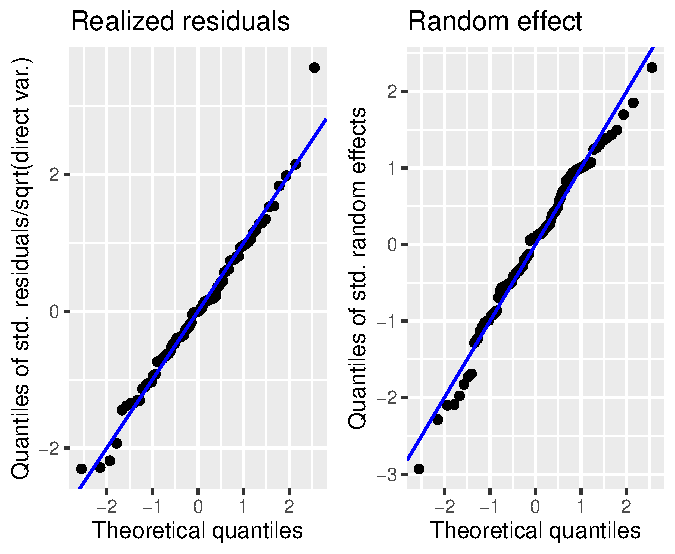
\includegraphics[width=1\linewidth]{./figures/plot1}
		\caption{}
		\label{fig:plota}
	\end{subfigure}
	\begin{subfigure}{0.48\textwidth}
		\centering
		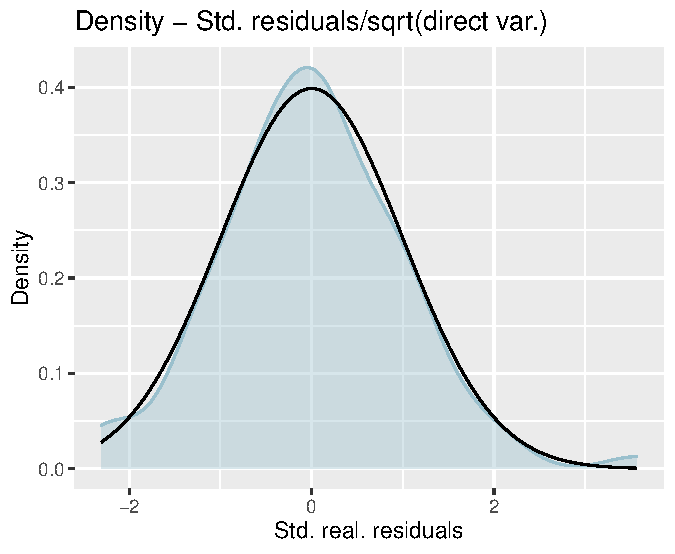
\includegraphics[width=1\linewidth]{./figures/plot2}
		\caption{}
		\label{fig:plotb}
	\end{subfigure}
	\begin{subfigure}{0.48\textwidth}
		\centering
		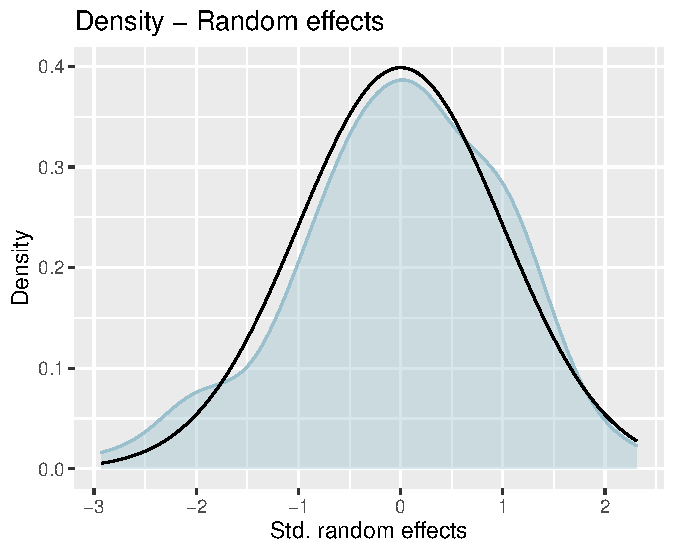
\includegraphics[width=1\linewidth]{./figures/plot3}
		\caption{}
		\label{fig:plotc}
	\end{subfigure}
	\caption{Output of \code{plot(fh\_std)}: (\subref{fig:plota}) normal quantile-quantile
		(Q-Q) plots of the standardized realized residuals
		and random effects, (\subref{fig:plotb}) and (\subref{fig:plotc}): kernel densities
		of the distribution of the standardized realized residuals
		and random effects (blue) in comparison to a standard normal distribution (black).}
	\label{fig:plot}
\end{figure}
%
\\ \newline
\textbf{Compare results with direct estimates} \\
The FH results should be consistent with the direct estimates for domains with
a small direct MSE and/or large sample sizes. Further, the precision of the direct
estimates should be improved by using auxiliary information. The comparison of
the direct and model-based (FH) estimates can be done graphically by the generic
function \code{compare\_plot}. For the \code{fh} method the required input argument
is an object of class \code{"fh"}. When the default settings of the command are
used, the output consists of two plots: a scatter plot proposed by \citet{Brown2001}
and a line plot. Besides the direct and FH estimates, the plot contains the fitted
regression and the identity line. These two lines should not differ too much. Preferably,
the model-based (FH) estimates should track the direct estimates within the line
plot especially for domains with a large sample size or small MSE of the direct
estimator. The points are ordered by decreasing MSE of the direct estimates. In
addition, the input arguments \code{MSE} and \code{CV} can be set to \code{TRUE}
leading to two extra plots, respectively. The MSE/CV estimates of the direct and model-based (FH) estimates are compared first via boxplots and second via
ordered scatter plots (ordered by increasing CV of the direct estimates). Like
for the \code{plot} command, a variety of customization options are offered, e.g.,
the label options (\code{label}), the format of the points (\code{shape}) and
the style of the line (\code{line\_type}).
\begin{example}
> compare_plot(fh_std, CV = TRUE, label = "no_title")
\end{example}
Except one high value, the fitted regression and identity line of the scatter
plot (Figure~\ref{fig:comparea}) are relatively close. Note that the high value
corresponds to the domain Eisenstadt (Stadt) with a very small sample size of 10
and the highest MSE of the direct estimates, so the direct estimator is very uncertain. Also the direct estimates are well tracked by the model-based (FH) estimates within the line plot (Figure~\ref{fig:compareb}). The boxplot (Figure~\ref{fig:comparee}) and the ordered scatter plot (Figure~\ref{fig:comparef}) show that the precision of the direct estimates could be improved by the usage of the FH model in terms of CVs. Additionally, all of the CV values are less than 20\% which is a common rule of the UK Office for National Statistics in order to determine whether estimation results should be published \citep{Miltiadou2020}.
\begin{figure}[h!]
	\centering
	\begin{subfigure}{0.48\textwidth}
		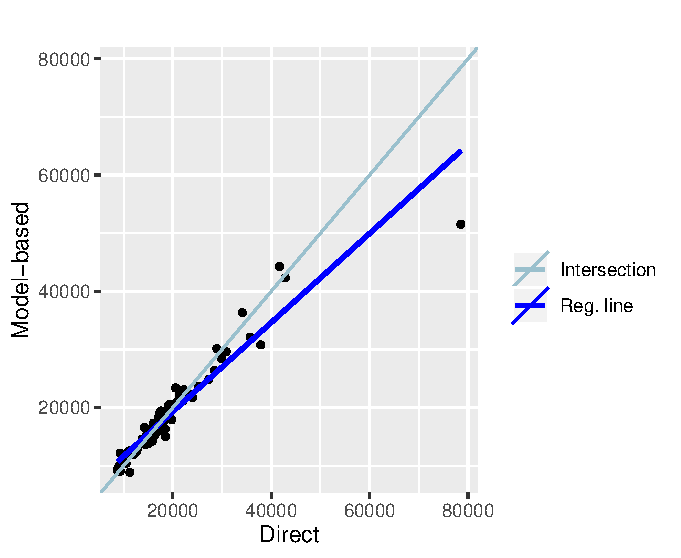
\includegraphics[width=7cm, keepaspectratio]{./figures/compare1}
		\caption{}
		\label{fig:comparea}
	\end{subfigure}
	\begin{subfigure}{0.48\textwidth}
		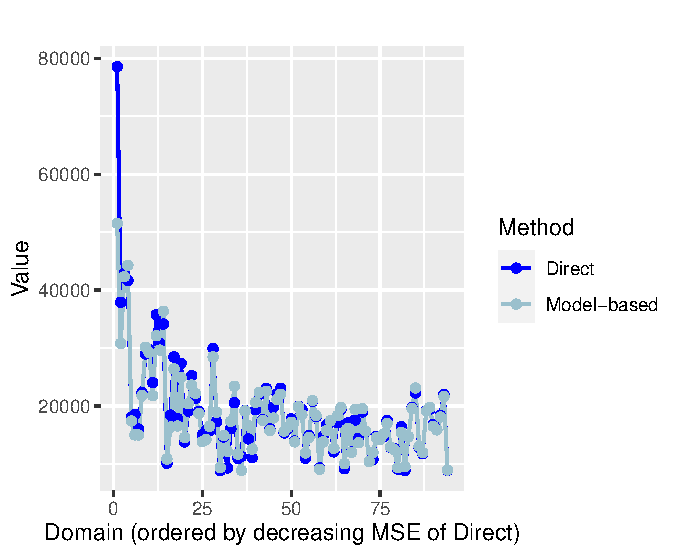
\includegraphics[width=7cm, keepaspectratio]{./figures/compare2}
		\caption{}
		\label{fig:compareb}
	\end{subfigure}
	\begin{subfigure}{0.48\textwidth}
		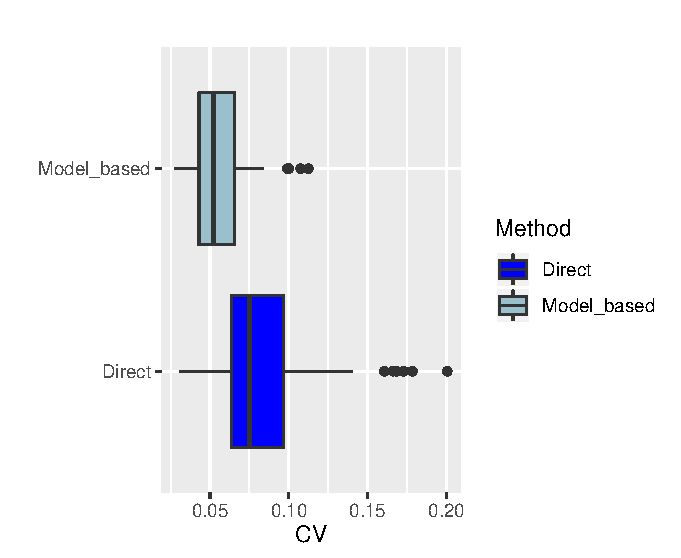
\includegraphics[width=7cm, keepaspectratio]{./figures/compare5}
		\caption{}
		\label{fig:comparee}
	\end{subfigure}
	\begin{subfigure}{0.48\textwidth}
		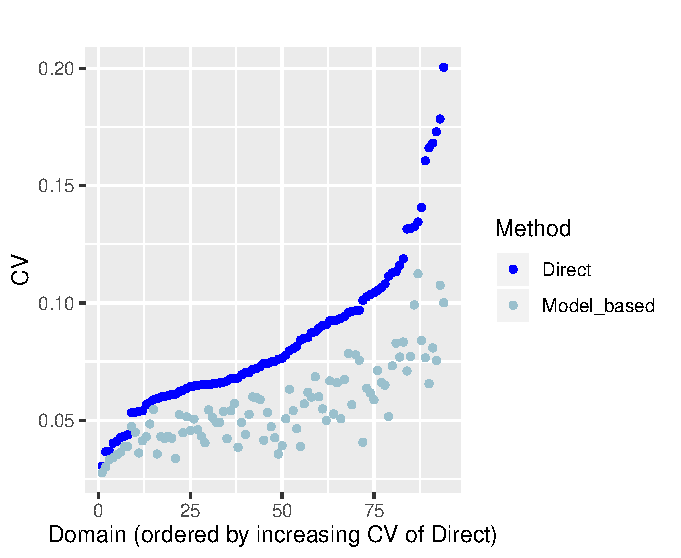
\includegraphics[width=7cm, keepaspectratio]{./figures/compare6}
		\caption{}
		\label{fig:comparef}
	\end{subfigure}
	\caption{Output of \code{compare\_plot(fh\_std)}: (\subref{fig:comparea}) and
		(\subref{fig:compareb}) scatter and line plots of direct and model-based point
		estimates, (\subref{fig:comparee}) and (\subref{fig:comparef}) boxplot and scatter
		plots of the CV estimates
		of the direct and model-based (FH) estimates.}
	\label{fig:compare}
\end{figure}
\newline
Further on, the function \code{compare} enables the user to compute a goodness of fit diagnostic \citep{Brown2001} and a correlation coefficient of the direct estimates and the estimates of the regression-synthetic part of the FH model \citep{Chandra2015}. Following \citet{Brown2001}, the difference between the model-based estimates and the direct estimates should not be significant (null hypothesis). The Wald test statistic is specified as
%
\begin{equation*}
W\left(\hat{\theta}_i^{\text{FH}}\right) = \sum_{i = 1}^{D} \frac{\left(\hat{\theta}_i^{\text{Dir}}-
	\hat{\theta}_i^{\text{FH}}\right)^2}{\widehat{\text{var}}\left(\hat{\theta}_i^{\text{Dir}}\right) + \widehat{\text{MSE}}\left(\hat{\theta}_i^{\text{FH}}\right)}
\end{equation*}
%
and is approximately $\chi^2$-distributed with $D$ degrees of freedom. When working with out-of-sample domains, those are not taken into account, because the direct estimates and their variances are missing. The input argument of function \code{compare} is an \code{"fh"} object.
\begin{example}
> compare(fh_std)

Brown test

Null hypothesis: EBLUP estimates do not differ significantly from the
      direct estimates

  W.value Df p.value
 46.97181 94 0.9999874

Correlation between synthetic part and direct estimator: 0.94
\end{example}
The results of the goodness of fit statistic and the correlation coefficient confirm what the scatter and the line plot already indicated. In the example the null hypothesis is not rejected and the correlation coefficient indicates a strong positive correlation (0.94) between the direct and model-based (FH) estimates.
\\ \newline
\textbf{Benchmarking for consistent estimates} \\
The idea of benchmarking is that the aggregated FH estimates should sum up to estimates of a higher regional level ($\tau$):
%
\begin{equation*}
\sum_{i=1}^{D} \xi_{i} \hat{\theta}_{i}^{\text{FH, bench}} = \tau,
\end{equation*}
%
where $\xi_{i}$ stands for the share of the population size of each area in the total population size ($N_{i}/N$).
In our example, the EBLUP estimates could get aggregated on a national level and then compared to or benchmarked with the Austrian mean equivalized income. The \pkg{emdi} package contains a benchmark function that allows the user to select three different options suggested by \citet{Datta2011b}. A general estimator of the three options can be written as follows:
%
\begin{equation*}
\hat{\theta}_{i}^{\text{FH, bench}} = \hat{\theta}_{i}^{\text{FH}} + \left( \sum_{i=1}^{D} \frac{\xi_{i}^2}{\phi_{i}} \right)^{-1} \left( \tau - \sum_{i=1}^{D} \xi_{i}\hat{\theta}_{i}^{\text{FH}}  \right) \frac{\xi_{i}}{\phi_{i}}.
\end{equation*}
%
Depending on the weight $\phi_{i}$, the formula leads to different benchmarking options.  If $\phi_{i}$ equals $\xi_{i}$, all FH estimates are adjusted by the same value (\code{raking}). A ratio adjustment (\code{ratio}) is being conducted if $\phi_{i} = \xi_{i}/\hat{\theta}_{i}^{\text{FH}}$. For the last option (\code{MSE\_adj}), $\phi_{i} = \xi_{i}/{\widehat{\text{MSE}}\left(\hat{\theta}_{i}^{\text{FH}}\right)}$. While the first option is a relatively naive approach, the latter two conduct larger adjustments for the areas with larger FH and MSE estimates, respectively. Thus, for the benchmark function the following arguments have to be specified: an object of class \code{"fh"}, a \code{benchmark} value, a vector containing the $\xi_{i}$s (\code{share}) and the \code{type} of benchmarking. The output is a data frame with an extra column \code{FH\_Bench} for the benchmarked EBLUP values. If the optional argument \code{overwrite} is set to \code{TRUE}, the benchmarked results are added to the \code{"fh"} object and the MSE estimates of the non benchmarked FH estimates are set to \code{NULL}.
For the used example, the benchmark value is calculated by taking the mean of the variable \code{eqIncome} of the \file{eusilcA\_smp} data frame. The $\xi_{i}$s can be found in \file{eusilcA\_popAgg} as \code{ratio\_n}.
\begin{example}
> fh_bench <- benchmark(fh_std, benchmark = 20140.09, share = eusilcA_popAgg$ratio_n,
+   type = "ratio")
> head(fh_bench)

              Domain   Direct       FH FH_Bench Out
1          Amstetten 14768.57 14242.04 14480.61   0
2              Baden 21995.72 21616.40 21978.49   0
3            Bludenz 12069.59 12680.38 12892.79   0
4     Braunau am Inn 10770.53 11925.82 12125.59   0
5            Bregenz 35731.20 32101.69 32639.43   0
6 Bruck-Mürzzuschlag 23027.37 22523.50 22900.79   0
\end{example}
It is recognizable that for the first six Austrian districts the original estimates are slightly modified by the benchmarking.
\\ \newline
\textbf{Extract and visualize the results} \\
To gain an overview of the point, MSE and CV results of the direct estimates compared to the model-based (FH) results the generic function \code{estimators} \citep{emdi2019} can be used, but differences among areas or hotspots of special interest are usually easier to detect on maps. With function \code{map\_plot}, the \pkg{emdi} package offers a user-friendly way to produce maps since creating maps can often become a time consuming task. The input arguments mainly consist of an object of class \code{"emdi"} and a spatial polygon of a shape file. The only issue that might come up is if domain identifiers in the data do not match to the respective identifiers of the shape file. In those cases, the input argument \code{map\_tab} is required, which is a data frame that contains the matching of the domain indentifiers of the population and the shape file data sets. For detailed instructions, we refer to \citet{emdi2019} and to the help page of function \code{map\_plot}.

For producing maps of the 94 Austrian districts, the Austrian shape file has to be loaded. In addition to the \code{"emdi"} object, the \code{"SpatialPolygonsDataFrame"} object (\code{map\_obj}) and a domain indicator (\code{map\_dom\_id}) have to be specified. The \code{map\_tab} argument is not necessary since the identifiers match in our example. To allow for an easier comparison of the results, we adjust the scales of the maps using the \code{scale\_points} argument.
\begin{example}
> load_shapeaustria()
> map_plot(object = fh_std, MSE = TRUE, map_obj = shape_austria_dis,
+   map_dom_id = "PB", scale_points = list(Direct = list(
+   ind = c(8000, 60000), MSE = c(200000, 10000000)), FH = list(
+   ind = c(8000, 60000), MSE = c(200000, 10000000))))
\end{example}
\begin{figure}[H]
	\begin{subfigure}[t]{0.49\textwidth}
		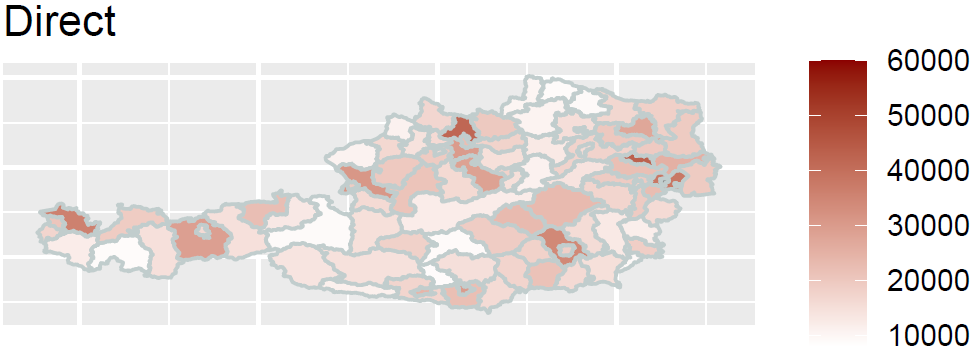
\includegraphics[width=\textwidth]{figures/map1.png}
		\caption{}
		\label{fig:mapa}
	\end{subfigure}\hfill%
	\begin{subfigure}[t]{0.49\textwidth}
		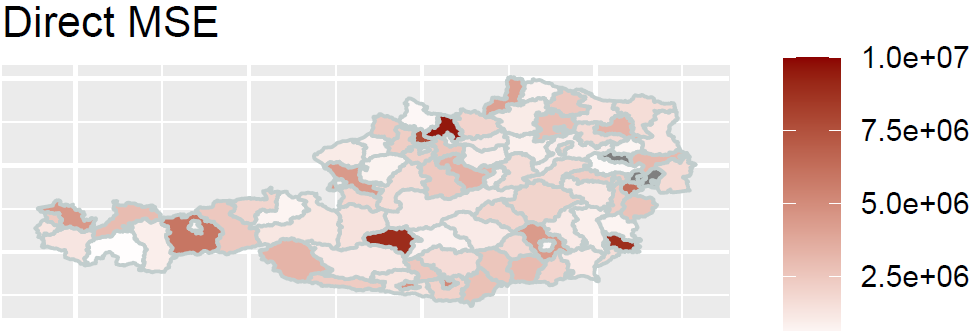
\includegraphics[width=\textwidth]{figures/map2.png}
		\caption{}
		\label{fig:mapb}
	\end{subfigure}\\[5pt]%
	%\centering
	\begin{subfigure}[t]{0.49\textwidth}
		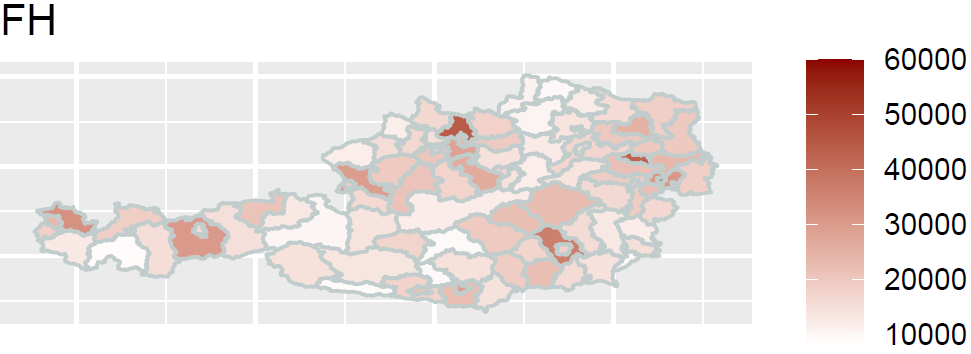
\includegraphics[width=\textwidth]{figures/map3.png}
		\caption{}
		\label{fig:mapc}
	\end{subfigure}\hfill%
	\begin{subfigure}[t]{0.49\textwidth}
		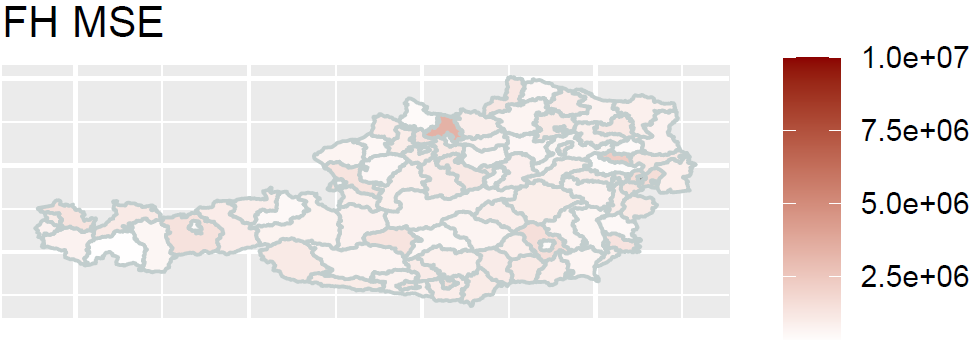
\includegraphics[width=\textwidth]{figures/map4.png}
		\caption{}
		\label{fig:mapd}
	\end{subfigure}%
	\caption{Output of \code{map\_plot}: Maps of the direct and FH estimates ((\subref{fig:mapa}) and (\subref{fig:mapc})) with corresponding MSE estimates ((\subref{fig:mapb}) and (\subref{fig:mapd})).}
	\label{fig:mapplot}
\end{figure}
Figures~\ref{fig:mapa} and~\ref{fig:mapc} show the distribution of the estimated
(direct vs. model-based) equivalized income across Austria. It is striking that
white and light red tones dominate the map, indicating relatively low mean
incomes of the districts. But in contrast, districts Eisenstadt
(Stadt), Urfahr-Umgebung and M\"odling stand out having the largest incomes.
Urfahr-Umgebung is also eye-catching when having a look at the MSE estimates
(Figures~\ref{fig:mapb} and~\ref{fig:mapd}). The MSE of the direct and the FH
estimates are quite high. Probably a single wealthy household raised the mean
income and also the variance. Figure~\ref{fig:mapb} contains some districts with
MSEs larger than the customized scaling (gray areas). Without the scaling it would
have been hard to identify any differences in Figure~\ref{fig:mapd}.	
\\ \newline
\textbf{Export the results} \\
Some users might have an interest to store the results separately or to use them
for presentations. Excel and OpenDocument Spreadsheets provide many opportunities for that. In contrast
to some existing R packages, the \pkg{emdi} functions \code{write.excel}/\code{write.ods}
do not only export the estimation results, but also the output of \code{summary}. Usage of the functions is comprehensively described in \citet{emdi2019}.

\subsection{Estimation of the extended area-level models} \label{sec:functionalityext}
\textbf{FH model with transformation} \\
If the indicator of interest needs a transformation, either log or arcsin, in addition to the function used in the previous subsection, the arguments \code{transformation} and \code{backtransformation} must be specified. If, for example, the share of households per area that earn more than the national median income (\code{MTMED}) is the indicator of interest, an arcsin transformation can be used. The bias-corrected back-transformation \code{bc} is chosen in the example. Two more arguments are needed when using an arcsin transformation: the name of the variable describing the effective sample sizes (\code{eff\_smpsize}) which needs to be contained in the \code{combined\_data} frame. Because of having chosen the bias-corrected back-transformation, the only possible \code{mse\_type} is \code{boot}, if the MSE estimation is activated.
\begin{example}
> fh_arcsin <- fh(fixed = MTMED ~ cash + age_ben + rent + house_allow,
+   vardir = "Var_MTMED", combined_data = combined_data, domains = "Domain",
+   transformation = "arcsin", backtransformation = "bc", eff_smpsize = "n",
+   MSE = TRUE, mse_type = "boot")
\end{example}
\textbf{Spatial FH model} \\
If the spatial correlation tests indicated a spatial correlation of the domains, a spatial FH model for incorporating the spatial structure in the model could be used. For that, the \code{correlation} has to be set to \code{spatial} and the example proximity matrix has to be given to the model within the \code{corMatrix} argument. The possible variance estimation methods are \code{ml} and \code{reml}.
\begin{example}
> fh_spatial <- fh(fixed = Mean ~ cash + self_empl, vardir = "Var_Mean",
+   combined_data = combined_data, domains = "Domain", correlation = "spatial",
+   corMatrix = eusilcA_prox, MSE = TRUE)
\end{example}
\textbf{Robust FH model} \\
If extreme values could influence the estimation, the application of a robust model might be appropriate. Within the robust framework, package \pkg{emdi} allows the user to choose between a standard and a spatial model (defaults to \code{correlation} = \code{"no"}). The estimation method must be \code{reblup} or \code{reblupbc} which includes a bias correction that can be modified by the argument \code{mult\_constant}. Further, the tuning constant \code{k} defaults to 1.345 as proposed by \citet{Sinha2009} and \citet{Warnholz2016} and can be changed if desired. The functions of the package \pkg{saeRobust} are utilized for the robust extensions. An exemplary call with pseudolinear MSE estimation looks like this:
\begin{example}
> fh_robust <- fh(fixed = Mean ~ cash + self_empl, vardir = "Var_Mean",
+   combined_data = combined_data, domains = "Domain", method = "reblup",
+   MSE = TRUE, mse_type = "pseudo")
\end{example}
\textbf{Measurement error model} \\
If other data sources than register data, e.g., data from larger surveys or big data sources are used as auxiliary information, the ME model should be applied. For the estimation of the ME model, the model fitting method must be set to \code{me} and the only possible MSE estimation method is \code{jackknife}. The most complex input argument consists of the creation of the MSE array \code{Ci}. The variability of the auxiliary variables that is taken into account by the ME model is expressed by the variance-covariance matrices per domain (\code{Ci}). For example, for three covariates a, b and c the array should look like
%
\begin{equation*}
\boldsymbol{C}_i = \left( \begin{array}{rrrr}
0 & 0 & 0 & 0 \\
0 & \text{var}_i(a) & \text{cov}_i(a,b) & \text{cov}_i(a,c) \\
0 & \text{cov}_i(a,b) & \text{var}_i(b) & \text{cov}_i(b,c) \\
0 & \text{cov}_i(a,c) & \text{cov}_i(b,c) & \text{var}_i(c) \\
\end{array}\right),
\text{   } i = 1,...,D.
\end{equation*}
%
The first row and column contain zeros, because the intercept is considered. The variances and covariances can be computed by standard approaches like, for example, the Horvitz-Thompson estimator.

For the Austrian EUSILC data example, the equalized income can also be explained by a variable of the sample data set. The code below demonstrates how the MSE array \code{Ci} is created for one covariate (variable \code{Cash} and its variance \code{Var\_Cash}) and how the final ME model is built.
\begin{example}
> P <- 1
> M <- 94
> Ci_array <- array(data = 0, dim = c(P + 1, P + 1, M))
> Ci_array[2,2, ] <- eusilcA_smpAgg$Var_Cash

> fh_yl <- fh(fixed = Mean ~ Cash, vardir = "Var_Mean",
+   combined_data = eusilcA_smpAgg, domains = "Domain", method = "me",
+   Ci = Ci_array, MSE = TRUE, mse_type = "jackknife")
\end{example}
\section[Conclusion and outlook]{Conclusion and outlook}\label{sec:concl}
In this paper, we have presented how the \pkg{emdi} package version 1.1.7 has been extended with various area-level models. Along with the well-known FH model, adjusted variance estimation methods and transformation options are offered to the user. In addition, spatial, robust, and ME model extensions of the standard model allow the user to address various issues that arise in practical data applications. All of these methods can be estimated conveniently by using a single function that provides EBLUP and the respective MSE estimates to measure their precision. Especially in the section~\nameref{sec:functionality}, it is clear that the package does not only contain tools for estimation of the different SAE models. Instead, it additionally provides user-friendly tools to enable a whole data analysis procedure: 1. starting with model building and estimation, moving on to 2. model assessment and diagnostics, 3. presentation of the results, and finishing with 4. exporting the results to Excel or OpenDocument Spreadsheet.

For future package versions, it is planned to expand the options in the field of area-level models.  In some practical applications, the incorporation of random effects is redundant. Therefore, an area-level estimator that considers a preliminary testing for the random effects following \citet{Molina2015a} will be included. Since version 2.0.0 \pkg{emdi} accounts for spatial structures of the random effects. Future developments may also account for out-of-sample EBLUP and MSE estimation for the spatial model proposed by \citet{Saei2005} and for temporal and spatio-temporal extensions \citep{Rao1994, Marhuenda2013}. For the existing ME model, a bootstrap MSE estimation option may  be added to the package since the Jackknife MSE estimator may produce negative MSE estimates \citep{Marchetti2015}. Furthermore, cross-validation options additional to the model assessment via information criteria and the $R^2$ will be investigated.
\section{Acknowledgments}\label{sec:Acknowledgments}
The work of Kreutzmann and Schmid has been supported by the German Research Foundation within the project QUESSAMI (281573942) and by the MIUR-DAAD Joint Mobility Program (57265468). The numerical results are not official estimates and are only produced for illustrating the methods.
The authors are indebted to the Editor-in-Chief, Associate Editor and the referees for comments that significantly improved the article.

\bibliography{harmening-kreutzmann-schmidt-salvati-schmid}

\newpage
\section{Appendix A: Area-level model options and corresponding input arguments} \label{sec:AppendixA}
%
\begin{figure}[h!]
	\centering
		\begin{subfigure}{\textwidth}
			\begin{adjustbox}{max width=\linewidth, scale=.99}
	\begin{tikzpicture}[node distance = 2cm, auto]
	% Transformation
	% Node
	\node [text width = 8em] (trans) {\textbf{FH model with transformation}};
	% Level 1: Transformation type
\node [below right of = trans, node distance = 1cm] (transtype) {transformation};
\node [block, below of = trans] (log) {\code{log}};
\node [block, right of = log, node distance = 8cm] (arcsin) {\code{arcsin}};
% Level 2: Backtransformation type
\node [block2, below of = log, node distance = 2.5cm] (crude) {crude bias-correction: \code{bc\_crude}};
\node [block2, right of = crude, node distance = 4cm] (sm) {Slud and Maiti bias-correction: \code{bc\_sm}};
\node[above of = sm, node distance = 1.5cm] (backtransf) {backtransformation};
\node [block2, right of = sm, node distance = 4cm] (naive) {Naive back-transformation: \code{naive}};
\node [block2, right of = naive, node distance = 4cm] (sm2) {general bias-correction: \code{bc}};
% Level 3: MSE
\node [block2, below of = crude, node distance = 2.5cm] (crudeMSE) {crude back-transf. Datta-Lahiri/ Prasad-Rao MSE: \code{analytical}};
\node [block2,below of = sm, node distance = 2.5cm] (smMSE) {Slud-Maiti analytical MSE: \code{analytical}};
\node [block2,below of = naive, node distance = 2.5cm] (jackknife) {(weighted) Jackknife MSE: (\code{weighted\_}) \code{jackknife}};
\node [block2, below of = sm2, node distance = 2.5cm] (bootstrap) {bootstrap MSE: \code{boot}};		
% draw
\draw [arrow] (trans) -- (log);
\draw [arrow] (trans) -- (arcsin);
\draw [arrow] (log) -- (crude);
\draw [arrow] (log) -- (sm);
\draw [arrow] (arcsin) -- (naive);
\draw [arrow] (arcsin) -- (sm2);
\draw (crude) -- (crudeMSE);
\draw (sm) -- (smMSE);
\draw [arrow] (naive) -- (jackknife);
\draw [arrow] (naive) -- (bootstrap);
\draw (sm2) -- (bootstrap);
	
	\end{tikzpicture}
	\end{adjustbox}
	\label{fig:flowtransformation}
\end{subfigure}
	\par\bigskip
\begin{subfigure}{\textwidth}
	\begin{adjustbox}{max width=\linewidth, scale=.99}
		\begin{tikzpicture}[node distance = 2cm, auto]
		% Spatial FH
		% Node
		\node (spatial) {\textbf{Spatial FH model}};
		% Level 1: Variance
		\node [below right of = spatial, node distance = 1cm] (variance) {method};
		\node [block, below of = spatial] (spatialML) {\code{ml}};
		\node [block, right of = spatialML, node distance = 5cm] (spatialREML) {\code{reml}};
		% Level 2: MSE
		\node [block2, below of = spatialML, text width = 11em, minimum height=6em] (spatialanalytical) {analytical MSE: \code{analytical}};
		\node [block2, below of = spatialREML, text width = 11em, minimum height=6em] (spatialnonparboot) {parametric bootstrap MSE: \code{spatialparboot}};
		\node [block2, right of = spatialnonparboot, node distance = 5cm, text width = 11em, minimum height=6em] (spatialparboot) {nonparametric bootstrap MSE: \code{spatialnonparboot}};
		% draw
		\draw [arrow] (spatial) -- (spatialML);
		\draw [arrow] (spatial) -- (spatialREML);
		\draw [arrow] (spatialML) -- (spatialanalytical);
		\draw [arrow] (spatialML) -- (spatialnonparboot);
		\draw [arrow] (spatialREML) -- (spatialanalytical);
		\draw [arrow] (spatialREML) -- (spatialnonparboot);
		\draw [arrow] (spatialREML) -- (spatialparboot);
		
		\end{tikzpicture}
	\end{adjustbox}
	\label{fig:flowspatial}
\end{subfigure}
\par\bigskip
\begin{subfigure}[t]{0.5\textwidth}
	\centering
	\begin{tikzpicture}[node distance = 2cm, auto]
	% Robust FH
	% Node
	\node (robust) {\textbf{Robust FH model}};
	% Level 1: Correlation
	\node [below right of = robust, node distance = 1cm] (correlation) {correlation};
	\node [block, below of = robust] (nocor) {\code{no}};
	\node [block, right of = nocor, node distance = 5cm] (spatialcor) {\code{spatial}};
	% Level 2: MSE
	\node [block, below of = nocor] (pseudoMSE) {pseudo linearisation MSE: \code{pseudo}};
	\node [block, below of = spatialcor] (bootMSE) {parametric bootstrap MSE: \code{boot}};
	% draw
	\draw [arrow] (robust) -- (nocor);
	\draw [arrow] (robust) -- (spatialcor);
	\draw [arrow] (nocor) -- (pseudoMSE);
	\draw [arrow] (nocor) -- (bootMSE);
	\draw [arrow] (spatialcor) -- (pseudoMSE);
	\draw [arrow] (spatialcor) -- (bootMSE);
	
	\end{tikzpicture}
	\label{fig:flowrobust}
\end{subfigure}%
\begin{subfigure}[t]{0.49\textwidth}
	\centering
	\begin{tikzpicture}[node distance = 2cm, auto]
	% Ybarra-Lohr
	% Node
	\node (ybarra) {\textbf{ME model}};
	% Level 1: Variance
	\node [below right of = ybarra, node distance = 1cm] (variance) {method};
	\node [block, below of = ybarra, text width = 10em] (moment) {measurement error model: \code{ME}};
	% Level 2: MSE
	\node [block, below of = moment, text width = 10em] (ybarrajack) {Jackknife MSE: \code{jackknife}};
	% draw
	\draw  (ybarra) -- (moment);
	\draw  (moment) -- (ybarrajack);
	\end{tikzpicture}
	\label{fig:flowME}
\end{subfigure}
\caption{Overview of extended area-level models and combinations of estimation methods.}
\label{fig:flow}
\end{figure}
\newpage
\begin{table}[h!]
	\centering
	\begin{adjustbox}{width=0.92\textwidth}
	\begin{tabularx}{\linewidth}{@{\extracolsep{\fill}}*1l @{}C @{}C @{}C @{}C @{}C}
		\toprule
		Argument & \multicolumn{5}{c}{FH model} \\
		& Standard  & Transformed & Spatial & Robust & ME\\ \midrule
		\code{fixed} & $\surd$ & $\surd$ & $\surd$ & $\surd$ & $\surd$ \\
\code{vardir} &  $\surd$ & $\surd$ & $\surd$  & $\surd$ & $\surd$\\
\code{combined\_data} &  $\surd$ & $\surd$ & $\surd$  & $\surd$ & $\surd$\\
\code{domains}  & ($\surd$) & ($\surd$) & ($\surd$) & ($\surd$) & ($\surd$) \\
\code{method} & $\surd$ & $\surd$ & $\surd$ & $\surd$ & $\surd$ \\
\code{interval} &  ($\surd$) & ($\surd$) &   & & \\
\code{k} &   &  &   & $\surd$ & \\
\code{mult\_constant}  &  &  &   &  $\surd$ &  \\
\code{transformation} & $\surd$ & $\surd$ & $\surd$  & $\surd$ & $\surd$\\
\code{backtransformation}  &  & $\surd$ &   &  & \\
\code{eff\_smpsize} \small{(only if} & & $\surd$  &  &   &  \\
\hspace{0.1cm} \small{\code{transformation = "arcsin"})} & & &  &   &  \\
\code{correlation} & $\surd$ & $\surd$ & $\surd$  & $\surd$ & $\surd$\\
\code{corMatrix} \small{(only if} &   &  &  $\surd$ & $\surd$  &  \\
\hspace{0.1cm} \small{\code{correlation = "spatial"})} & & &  &   &  \\
\code{Ci}  &  &  &   &   & $\surd$ \\
\code{tol} &  &  & $\surd$  & $\surd$ & $\surd$\\
\code{maxit}  & &  & $\surd$ & $\surd$ & $\surd$ \\
\code{MSE} & $\surd$ & $\surd$ & $\surd$ & $\surd$ & $\surd$ \\
\code{mse\_type} \small{(only if \code{MSE = TRUE})} & $\surd$ & $\surd$ & $\surd$ & $\surd$ & $\surd$ \\
\code{B} & ($\surd$) & $\surd$  & $\surd$ & $\surd$ &  \\
\code{seed}  & ($\surd$) & ($\surd$) & ($\surd$) & ($\surd$) &  \\
		\bottomrule
	\end{tabularx}
\end{adjustbox}
	\caption{Required $\surd$ and optional ($\surd$) input arguments of function \code{fh} for the different area-levels models. \code{B}: Only if bootstrap MSE is chosen. When the standard FH model is applied, \code{B} is required for the computation of the information criteria by \citet{Marhuenda2014} (optionally).}
	\label{tab:inputarg}
\end{table}
\section{Appendix B: Output of the model component} \label{sec:AppendixB}
\begin{table}[h!]
	\centering
	\begin{adjustbox}{width=0.92\textwidth}
	\begin{tabularx}{\linewidth}{@{\extracolsep{\fill}}X @{}X @{}g @{}f @{}g @{}g @{}s}
		\toprule
		Name & Short description & \multicolumn{5}{c} {Available for} \\
		& & Standard  & Transformed & Spatial & Robust & ME\\ \midrule
		\code{coefficients} & \raggedright{Estimated regression coefficients} & $\surd$ & $\surd$ & $\surd$ & $\surd$ & $\surd$ \\
		\code{variance} & \raggedright{Estimated variance of the random effects/ estimated spatial correlation parameter} & $\surd$ & $\surd$ & $\surd$  & $\surd$ & $\surd$\\
		\code{random\_effects} & \raggedright{Random effects per domain} & $\surd$ & $\surd$ & $\surd$  & $\surd$ & $\surd$\\
		\code{real\_residuals} & \raggedright{Realized residuals per domain}  & $\surd$ & $\surd$ & $\surd$ & $\surd$ & $\surd$ \\
		\code{std\_real\_residuals} & \raggedright{Standardized realized residuals per domain} & $\surd$ & $\surd$ & $\surd$ & $\surd$ & $\surd$ \\
		\code{gamma} & \raggedright{Shrinkage factors per domain} & $\surd$ & $\surd$ &   & & $\surd$ \\
		\code{model\_select} & \raggedright{Model selection and accuracy criteria} & $\surd$ & $\surd$ & $\surd$  & & \\
		\code{correlation}  & \raggedright{Selected correlation structure of the random effects} & $\surd$ & $\surd$ & $\surd$  &  $\surd$ & $\surd$ \\
		\code{k}  & \raggedright{Tuning constant} &  & &   &  $\surd$ &  \\
		\code{mult\_constant}  & \raggedright{Multiplier constant for bias correction} &  & &   &  $\surd$ &  \\
		\code{seed}  & \raggedright{Seed of the random number generator} &  $\surd$ &  $\surd$ &   $\surd$ &  $\surd$ &  \\\bottomrule
	\end{tabularx}
\end{adjustbox}
	\caption{Components of the output component \code{model} for models of class \code{"fh"}.}
	\label{tab:modelcomp}
\end{table}
\newpage
\section{Reproducibility}
For the computation of the results in this paper we worked with R version 4.2.2  on a 64-bit platform under Microsoft Windows 10 with the installed packages listed in Table~\ref{tab:Rpackages}. Using the package \CRANpkg{packrat} \citep{Ushey2018} a snapshot of the corresponding repository was created that is available from the GitHub folder (\url{https://github.com/SoerenPannier/emdi.git}). We suggest the following steps:
\begin{itemize}
	\item Install Git.
	\item Create a new project in RStudio.
	\item Choose checkout from version control and select Git.
	\item Insert the repository URL: \url{https://github.com/SoerenPannier/emdi.git}.
	\item Let \pkg{packrat} complete the initialization process.
	\item Restart RStudio.
	\item Enter the R command \code{packrat::restore()}.
	\item After finishing the installation process all packages are installed as provided in Table~\ref{tab:Rpackages}.
\end{itemize}
%
\begin{table}[h]
	\centering
	%\scalebox{1}{
		\begin{tabular}{lr|lr|lr}
			\toprule
			Package & Version & Package & Version & Package & Version \\
			\midrule
			aoos & 0.5.0 & highr & 0.9 & RColorBrewer & 1.1-3 \\
			assertthat & 0.2.1 & HLMdiag & 0.5.0 & Rcpp & 1.0.9 \\
			backports & 1.4.1 & hms & 1.1.1 & RcppArmadillo & 0.11.2.0.0 \\
			BBmisc & 1.12 & isoband & 0.2.5 & readODS & 1.7.0 \\
			bit & 4.0.4 & janitor & 2.1.0 & readr & 2.1.2 \\
			bit64 & 4.0.5 & jsonlite & 1.8.0 & rematch & 1.0.1 \\
			boot & 1.3-28 & knitr & 1.39 & rematch2 & 2.1.2 \\
			brew & 1.0-7 & labeling & 0.4.2 & reshape2 & 1.4.4 \\
			brio & 1.1.3 & laeken & 0.5.2 & rgeos & 0.5-9 \\
			cachem & 1.0.6 & lifecycle & 1.0.1 & rlang & 1.0.4 \\
			callr & 3.7.1 & lubridate & 1.8.0 & roxygen2 & 7.2.1 \\
			cellranger & 1.1.0 & magrittr & 2.0.3 & rprojroot & 2.0.3 \\
			checkmate & 2.1.0 & maptools & 1.1-4 & s2 & 1.1.0 \\
			classInt & 0.4-7 & MASS & 7.3-58 & saeRobust & 0.3.0 \\
			cli & 3.3.0 & memoise & 2.0.1 & scales & 1.2.0 \\
			clipr & 0.8.0 & modules & 0.10.0 & sf & 1.0-8 \\
			colorspace & 2.0-3 & moments & 0.14.1 & simFrame & 0.5.4 \\
			commonmark & 1.8.0 & MuMIn & 1.47.1 & snakecase & 0.11.0 \\
			cpp11 & 0.4.2 & munsell & 0.5.0 & sp & 1.5-0 \\
			crayon & 1.5.1 & nlme & 3.1-158 & spData & 2.0.1 \\
			data.table & 1.14.2 & openxlsx & 4.2.5 & spdep & 1.2-4 \\
			DBI & 1.1.3 & operator.tools & 1.6.3 & stringi & 1.7.8 \\
			deldir & 1.0-6 & packrat & 0.8.1 & stringr & 1.4.0 \\
			desc & 1.4.1 & parallelMap & 1.5.1 & terra & 1.5-34 \\
			diagonals & 6.4.0 & pbapply & 1.5-0 & testthat & 3.1.4 \\
			diffobj & 0.3.5 & pillar & 1.8.0 & tibble & 3.1.8 \\
			digest & 0.6.29 & pkgconfig & 2.0.3 & tidyr & 1.2.0 \\
			dplyr & 1.0.9 & pkgload & 1.3.0 & tidyselect & 1.1.2 \\
			e1071 & 1.7-11 & plyr & 1.8.7 & tzdb & 0.3.0 \\
			ellipsis & 0.3.2 & praise & 1.0.0 & units & 0.8-0 \\
			emdi & 2.1.3 & prettyunits & 1.1.1 & utf8 & 1.2.2 \\
			evaluate & 0.15 & processx & 3.7.0 & vctrs & 0.4.1 \\
			fansi & 1.0.3 & progress & 1.2.2 & viridisLite & 0.4.0 \\
			farver & 2.1.1 & proxy & 0.4-27 & vroom & 1.5.7 \\
			fastmap & 1.1.0 & ps & 1.7.1 & waldo & 0.4.0 \\
			formula.tools & 1.7.1 & purrr & 0.3.4 & withr & 2.5.0 \\
			fs & 1.5.2 & R.cache & 0.16.0 & wk & 0.6.0 \\
			generics & 0.1.3 & R.methodsS3 & 1.8.2 & xfun & 0.31 \\
			ggplot2 & 3.3.6 & R.oo & 1.25.0 & xml2 & 1.3.3 \\
			ggrepel & 0.9.1 & R.rsp & 0.45.0 & yaml & 2.3.5 \\
			glue & 1.6.2 & R.utils & 2.12.0 & zip & 2.2.0 \\
			gridExtra & 2.3 & R6 & 2.5.1 &   &   \\
			gtable & 0.3.0 & raster & 3.5-21 &  &  \\
			\bottomrule
		\end{tabular}
%	}
	\caption{Installed packages for the computation of the results in this paper.}\label{tab:Rpackages}
\end{table}

\address{Sylvia Harmening\\
  Institute for Statistics and Econometrics, School of Business \& Economics, Freie Universit\"at Berlin\\
  Garystr.~21, 14195 Berlin\\
  Germany\\
  \email{sylvia.harmening@fu-berlin.de}}

\address{Ann-Kristin Kreutzmann\\
	Institute for Statistics and Econometrics, School of Business \& Economics, Freie Universit\"at Berlin\\
	Garystr.~21, 14195 Berlin\\
	Germany\\
	\email{ann-kristin.kreutzmann@fu-berlin.de}}

\address{Sören Schmidt\\
	Institute for Statistics and Econometrics, School of Business \& Economics, Freie Universit\"at Berlin\\
	Garystr.~21, 14195 Berlin\\
	Germany\\
	\email{soeren.pannier@fu-berlin.de}}

\address{Nicola Salvati\\
	Department of Economics and Management, University of Pisa\\
	Via C. Ridolfi, 10 56124 Pisa\\
	Italy\\
	\email{nicola.salvati@unipi.it}}

\address{Timo Schmid \\
	Institute of Statistics, Otto-Friedrich-Universit\"at Bamberg \\
	Feldkirchenstr.~21, 96052 Bamberg\\
	Germany \\
	\email{timo.schmid@uni-bamberg.de}}
